\documentclass[a4paper,leqno,twocolumn]{article}
% ==== Inputs and Usepackages ====

\usepackage{tablefootnote}
\usepackage{enumerate}
\usepackage{float}
\usepackage{url}
\usepackage{hyperref}
\usepackage{dsfont}
\usepackage{mathrsfs}
\usepackage{amsmath}
\usepackage{amssymb}
\usepackage{amsthm}
\usepackage{amsfonts}
\usepackage{mathtools}
%\usepackage{mathabx}
\usepackage{MnSymbol}
\usepackage{xfrac}
\usepackage{nicefrac}
\usepackage{geometry}
\usepackage{graphicx}
\usepackage{graphics}
\usepackage{latexsym}
\usepackage{setspace}
\usepackage{tikz-cd}
\usepackage{tikz}
 \usetikzlibrary{matrix}
 \usetikzlibrary{calc}
 \usetikzlibrary{circuits.ee.IEC}
\usepackage{circuitikz}

\usepackage{a4wide}
\usepackage{fancybox}
\usepackage{fancyhdr}
\usepackage[utf8]{inputenc}




% ==== Page Settings ====

\hoffset = -1.2 in
\voffset = -0.3 in
\textwidth = 590pt
\textheight = 770pt
\setlength{\headheight}{20pt}
\setlength{\headwidth}{590pt}
\marginparwidth = 0 pt
\topmargin = -0.75 in
\setlength{\parindent}{0cm}


% ==== Presettings for files ====

\pagestyle{fancy}


\cfoot{\thepage}
\lfoot{\href{mailto:szekerb@student.ethz.ch}{szekerb@student.ethz.ch}}
\rfoot{Balázs Szekér, \today}
\lhead{Physics \uproman{3} Summary}

% ==== General Commands ====

\newcommand{\sframebox}[1]{
        \framebox[500pt][l]{\parbox{490pt}{
            #1
        }
    }

}

\newcommand{\cframebox}[2]{
        \fbox{\parbox{#1pt}{
            #2
        }
    }
}









% ====== Maths ======


% ==== Formats ====
\newcommand{\boldline}[1]{\textbf{\underline{#1}}}
\newcommand{\uproman}[1]{\uppercase\expandafter{\romannumeral#1}}
\newcommand{\lowroman}[1]{\romannumeral#1\relax}
\newcommand{\fat}[1]{\textbf{#1}}
\newcommand{\Loesung}{\begin{center}\textbf{Lösung}\end{center}}

\newcommand{\Korollar}[1]{\textbf{Korollar} \vspace{1\baselineskip} #1}
\newcommand{\Beispiel}[1]{\textbf{Beispiel} \vspace{1\baselineskip} #1}
\newcommand{\Beweis}[1]{\textbf{Beweis} \vspace{1\baselineskip} #1}
\newcommand{\Proposition}[1]{\textbf{Proposition} \vspace{1\baselineskip} #1}
\newcommand{\Satz}[1]{\textbf{Satz} \vspace{1\baselineskip} #1}
\newcommand{\Definition}[1]{\textbf{Definition} \vspace{1\baselineskip} #1}
\newcommand{\Lemma}[1]{\textbf{Lemma}\vspace{1\baselineskip} #1}
\newcommand{\Bemerkung}[1]{\textbf{Bemerkung} \vspace{1\baselineskip} #1}
\newcommand{\Theorem}[1]{\textbf{Theorem} \vspace{1\baselineskip} #1}




% ==== mathsymbols ====
\newcommand{\Q}{\mathbb{Q}}
\newcommand{\R}{\mathbb{R}}
\newcommand{\N}{\mathbb{N}}
\newcommand{\Z}{\mathbb{Z}}
\newcommand{\C}{\mathbb{C}}
\newcommand{\K}{\mathbb{K}}
\newcommand{\eS}{\mathbb{S}}
\newcommand{\X}{$X$ }
\newcommand{\Y}{$Y$ }
\newcommand{\x}{$x$ }
\newcommand{\y}{$y$ }
\newcommand{\B}{\mathcal{B}}
\newcommand{\A}{\mathcal{A}}
\renewcommand{\S}{\mathcal{S}}
\renewcommand{\P}{\mathcal{P}}



% ==== math operators ====
\newcommand{\klammer}[1]{\left( #1 \right)} 
\newcommand{\eckigeklammer}[1]{\left[ #1 \right]}
\newcommand{\geschwungeneklammer}[1]{\left\{ #1 \right\}}
\newcommand{\floor}[1]{\left\lfloor #1 \right\rfloor}
\newcommand{\ceil}[1]{\left\lceil #1 \right\rceil}
\newcommand{\scalprod}[2]{\left\langle #1 , #2 \right\rangle}
\newcommand{\abs}[1]{\left\vert #1 \right\vert} 
\newcommand{\Norm}[1]{\left\vert\left\vert #1 \right\vert\right\vert}
\newcommand{\intab}{\int_a^b}
\newcommand{\intii}{\int_{-\infty}^\infty} 
\newcommand{\cint}[2]{\int_{#1}^{#2}}
\newcommand{\csum}[2]{\sum_{#1}^{#2}}
\newcommand{\limes}[1]{\lim\limits_{#1}}
\newcommand{\limessup}[1]{\limsup\limits_{#1}}
\newcommand{\limesinf}[1]{\liminf\limits_{#1}}
\newcommand{\limesninf}{\limes{n \rightarrow \infty}}
\newcommand{\limsupninf}{\limessup{n \rightarrow \infty}}
\newcommand{\liminfninf}{\limesinf{n \rightarrow \infty}}
\newcommand{\standardNorm}{\Norm{ \ \cdot \ }}
\newcommand{\einsNorm}{\Norm{ \ \cdot \ }_1}
\newcommand{\zweiNorm}{\Norm{ \ \cdot \ }_2}
\newcommand{\Hom}{\text{Hom}}
\newcommand{\Mat}{\text{Mat}}
\newcommand{\grad}{\text{grad}}
\newcommand{\vol}{\text{vol}}
\newcommand{\supp}{\text{supp}}
\newcommand{\rot}{\text{rot}}
\renewcommand{\div}{\text{div}}



% ==== Analysis ====
\newcommand{\supremum}{\text{sup}}
\newcommand{\infimum}{\text{inf}}
\newcommand{\maximum}{\text{max}}
\newcommand{\minimum}{\text{min}}

\newcommand{\xinX}{$x \in X$ }
\newcommand{\yinY}{$y \in Y$ }
\newcommand{\xyinX}{$x,y \in X$ }
\newcommand{\yinX}{$y \in X$ }
\newcommand{\xinR}{$x \in \R$ }
\newcommand{\xyinR}{$x,y \in \R$ }
\newcommand{\zinC}{$z \in \C$ }
\newcommand{\ninN}{$n \in \N$ }
\newcommand{\NinN}{$N \in \N$}
\newcommand{\angeordneterK}{$(K,\leq)$ }
\newcommand{\xFolge}{(x_n)_{n=0}^{\infty}}
\newcommand{\yFolge}{(y_n)_{n=0}^{\infty}}
\newcommand{\zFolge}{(z_n)_{n=0}^{\infty}}
\newcommand{\aFolge}{(a_n)_{n=0}^{\infty}}
\newcommand{\fFolge}{(f_n)_{n=0}^{\infty}}

\newcommand{\XsubR}{$X \subset \R$ }
\newcommand{\XsubeqR}{$X \subseteq \R$ }

\newcommand{\XFam}{\mathcal{X}}
\newcommand{\PFam}{\mathcal{P}}

\newcommand{\offenesintervall}[2]{$\left( #1 , #2 \right)$ }
\newcommand{\abgeschlossenesintervall}[2]{$\left( #1 , #2 \right)$ }

\newcommand{\XTopRaum}{(X,\tau)}


% ==== Lineare Algebra ====
\newcommand{\vinV}{$v \in V$ }
\newcommand{\uinU}{$u \in U$ }
\newcommand{\winW}{$w \in W$ }
\newcommand{\vwinV}{$v,w \in V$ }

\newcommand{\BasisV}{v_1 , \dots , v_n}
\newcommand{\BasisU}{u_1 , \dots , u_n}
\newcommand{\BasisW}{w_1 , \dots , w_n}

\newcommand{\transpose}[1]{#1^t}
\newcommand{\inverse}[1]{#1^{-1}}
\newcommand{\ddvec}[3]{\left( #1,#2,#3 \right)}
\newcommand{\tdvec}[2]{\left( #1 , #2 \right)}

\newcommand{\Edrei}{\begin{pmatrix}
    1 & 0 & 0 \\
    0 & 1 & 0 \\
    0 & 0 & 1
\end{pmatrix}}

\newcommand{\id}{\text{id}}
\newcommand{\GL}{\text{GL}}
\newcommand{\End}{\text{End}}
\renewcommand{\Im}{\text{Im}}
\renewcommand{\Re}{\text{Re}}
\renewcommand{\ker}{\text{Ker}}
\newcommand{\rang}{\text{rang}}
\newcommand{\ad}{\text{ad}}
\newcommand{\Eig}{\text{Eig}}
\newcommand{\Bil}{\text{Bil}}
\newcommand{\sign}{\text{sign}}
\newcommand{\tr}{\text{tr}}



% ====== Physics ======

% ==== Physicssymbols ====
\newcommand{\epsilonnull}{\epsilon_0}
\newcommand{\munull}{\mu_0}
\newcommand{\rn}{r_0}
\newcommand{\Rn}{R_0}
\newcommand{\rhonull}{\rho_0}
\newcommand{\Rhonull}{\varrho_0}


% ==== Notation ====
\newcommand{\Etot}{E_{\text{Tot}}}
\newcommand{\Wtot}{W_{\text{Tot}}}
\newcommand{\Ftot}{F_{\text{Tot}}}
\newcommand{\vtot}{v_{\text{Tot}}}
\newcommand{\atot}{a_{\text{Tot}}}
\newcommand{\mtot}{m_{\text{Tot}}}
\newcommand{\Mtot}{M_{\text{Tot}}}

\newcommand{\Ekin}{E_{\text{Kin}}}
\newcommand{\Epot}{E_{\text{Pot}}}
\newcommand{\Edef}{E_{\text{Def}}}

\newcommand{\Fg}{F_g}
\newcommand{\FN}{F_N}
\newcommand{\Fz}{F_z}
\newcommand{\FC}{F_C}

\newcommand{\xn}{x_0}
\newcommand{\xN}{x_n}
\newcommand{\vn}{v_0}
\newcommand{\vN}{v_n}
\newcommand{\an}{a_0}
\newcommand{\aN}{a_n}

\newcommand{\dt}{\Delta t}
\newcommand{\dx}{\Delta x}
\newcommand{\dv}{\Delta v}
\newcommand{\da}{\Delta a}
\newcommand{\dE}{\Delta E}
\newcommand{\dW}{\Delta W}
\newcommand{\dF}{\Delta F}


% ==== Relativity ====
\newcommand{\relsqrt}{\sqrt{1-\frac{v^2}{c^2}}}
\newcommand{\relgamma}{\frac{1}{\relsqrt}}


% ==== Constants ====
\newcommand{\g}{9.81}





\renewcommand{\epsilon}{\varepsilon}
\clubpenalty = 10000
\widowpenalty = 10000
\usepackage[skins,theorems]{tcolorbox}

\begin{document}

\tcbset{highlight math style={enhanced, sharp corners=uphill,
  colframe=red!75!black,colback=red!5!white,arc=0pt,boxrule=1pt}}

\section{Wellen}

\vspace{1\baselineskip}

Die \fat{Wellenfunktion} ist gegeben durch $\xi = \xi (x,t) = f(x \pm v t)$.
Wobei "$+$" Verschiebung nach \underline{links} und "$-$" nach \underline{rechts}.

$v$ ist die \fat{Phasengeschwindigkeit}, welche die Geschwindigkeit einer Welle angibt,
mit der sich eine vorgegebene Phase bewegt.

\vspace{1\baselineskip}

Die \fat{Harmonische Wellenfunktion} ist gegeben durch
\[
  \xi(x,t) = \xi_0 \sin (k(x \pm vt)) = \xi_0 \sin (kx \pm \omega t) = \xi_0 e^{i (kx \pm \omega t)}
\]
wobei
\begin{itemize}
    \item $k$: \fat{Wellenzahl} resp. \fat{Wellenvektor} (Anzahl Wellen pro Längeneinheit) mit $[k]=\frac{1}{m}$ oder $\frac{\text{rad}}{m}$
    \item $\epsilon_0$: \fat{Amplitude} mit $[\xi_0] = m$
    \item $\lambda$: \fat{Wellenlänge} mit $[\lambda] = m$
    \item $\omega$: \fat{Frequenz} in $\frac{\text{rad}}{s}$ oder $\frac{1}{s}$
\end{itemize}
Zusammenhänge:
\begin{itemize}
    \item Frequenz: $\omega = k v$ und $2 \pi f = \omega$
    \item Wellenvektor: $k = \frac{2 \pi}{\lambda}$
    \item Periode: $T = \frac{2 \pi}{\omega} = \frac{1}{f}$
\end{itemize}

\vspace{1\baselineskip}

Die \fat{Wellengleichung} in einer Dimension lautet:
\[
  \frac{\partial^2 \xi}{\partial t^2} - v^2 \frac{\partial^2 \xi}{\partial x^2}  
\]
Wir unterscheiden zwei Arten von Wellen:
\begin{itemize}
    \item \fat{Transversale Welle}: $\xi (x,t) = A f(x-vt) \hat{z}$
    
            Auslenkung senkrecht zur Propagationsrichtung.
            
            Bsp: (elastische Seilwelle)
            $v = \pm \sqrt{\frac{S}{\mu}}$ mit $S=\frac{F}{A}=$ Zugspannung und $\mu=$ Dichte (Masse
            pro Volumenelement)

    \item \fat{Longitudale Welle}: $\xi (x,t) = A f(x-vt) \hat{x}$
    
            Auslenkung parallel zur Propagationsrichtung.

            Bsp: (Federkette oder Welle im Festkörper)
            $v= \pm \sqrt{\frac{E}{\rho}}$ mit $E= \frac{F}{A} \cdot \frac{l}{\Delta l}
            = \frac{\sigma}{\epsilon_l}$
            Elastizitätsmodul und $\rho= \frac{dm}{dV} = \frac{dm}{A \ dz} =$ Dichte
\end{itemize}

\vspace{1\baselineskip}

In einer \fat{ebenen Welle} ist die Phase an jedem Ort senkrecht zur Ausbreitungsrichtung
identisch: $\xi(x,y,z,t) = A f(kz-\omega t)$

\vspace{1\baselineskip}

\fat{Polarisation} von $\vec{A} e^{i (kz-\omega t)}$:
\begin{itemize}
    \item \fat{linear}: Welle schwingt in Ebene
    \item \fat{eliptisch}: Überlagerung von zwei linear polarisierten Wellen mit Phasenunterschied
    \item \fat{zirkulär polarisiert}: Spezialfall der eliptischen Welle mit
            Phasenunterschied $\Delta \delta = \frac{\pi}{2}$
\end{itemize}

\vspace{1\baselineskip}

\fat{Wellengleichung in 3D}: Für $\xi := \vec{\xi}(\vec{r},t) = \vec{A} e^{i (\vec{k} \cdot \vec{r} - \omega t)}$
\[
    \frac{1}{v^2} \frac{\partial^2 \xi}{\partial t^2} - \frac{\partial^2 \xi}{\partial x^2}
    \frac{\partial^2 \xi}{\partial y^2} - \frac{\partial^2 \xi}{\partial z^2} 
    = \frac{1}{v^2} \frac{\partial^2 \xi}{\partial t^2} - \Delta \xi
    = 0
\]

\pagebreak

\fat{Wellengleichung für Kugelwellen}:

Für $\xi := \vec{\xi}(\vec{r},t) = \vec{A} e^{i (\vec{k} \cdot \vec{r} - \omega t)}$
\[
    \frac{1}{v^2} \frac{\partial^2 \xi}{\partial t^2} = \klammer{\frac{\partial^2}{\partial r^2} + \frac{2}{r} \frac{\partial}{\partial r}} \xi
\]

\vspace{1\baselineskip}

\begin{minipage}{0.2\textwidth}
    \fat{kinetische \\ Energiedichte}:
    \[
        \frac{dT}{dV} = \frac{1}{2} \rho \klammer{\frac{\partial \vec{\xi}}{\partial t}}^2  
    \]
\end{minipage}
\begin{minipage}{0.2\textwidth}
    \fat{elastische \\ Energiedichte}:
    \[
          \frac{dE_{el}}{dV} = \frac{1}{2} E \klammer{\frac{\partial \vec{\xi}}{\partial x}}^2
    \]
\end{minipage}

\vspace{1\baselineskip}

\fat{Gesammtenergie}:
\[
    \frac{d W}{d V} = \frac{d E_{el}}{dV} + \frac{dT}{dV} =
    \rho v^2 \klammer{\frac{\partial f}{\partial u} \frac{\partial u}{\partial x}}^2  
\]
konkret für Welle $\xi(x,t)= A \cos (kx-\omega t)$ mit Phasengeschw. $v=\frac{\omega}{k}$
\[
    \frac{dW}{dV} =   \rho v^2 k^2 A^2 \sin^2 (kx-\omega t)
    = \rho \omega^2 A^2 \sin^2 (kx-\omega t)
\]

Wir definieren die \fat{mittlere Energiedichte} als:
\[
    \left\langle \frac{dW}{dV} \right\rangle  = \frac{1}{T} \int_0^T \frac{dW}{dV} (x,t) dt
    = \frac{1}{2} \rho \omega^2 A^2
\]

Die \fat{Energieflussdichte} (/der \fat{Poynting-Vektor}) $S$ ist diejenige Energie, welche pro
Zeit durch ein zum Fluss orthogonalen Flächenelement steht.
\[
    \vec{S} = \frac{d^2 W}{da \cdot dt} \cdot \frac{d \vec{a}}{\abs{d \vec{a}}}  
    \quad \text{ mit } \quad
    [S] = \frac{J}{m^2 s} = \frac{W}{m^2}
\]

Die \fat{Intensität} ist der Betrag von $S$: $I = \abs{S}$ und wird auch als
\fat{Energiestrom} bezeichnet. Die \fat{mittlere Intensität} ist:
\[
    \left\langle I \right\rangle = \frac{1}{2} \rho \omega^2 A^2 v
    = \frac{1}{2} \rho \frac{\omega^3}{k} A^2  
    = \frac{P}{A} = \frac{\text{Leistung}}{\text{Oberfläche}}
\]
Mittlerer Energiestrom der durch die gesammte Kugeloberfläche im Abstand $r$
hindurchtretenden Welle:
\[
    \dot{W} = \frac{1}{2} \rho \omega^2 \klammer{\frac{A_0}{r}}^2 \cdot v \cdot 4 \pi r^2  
\]

\vspace{1\baselineskip}

\fat{Superpositionsprinzip}: Summe zweier Wellen ist wieder eine Welle.
Hilfreiche Trigonometrische Additionstheoreme:
\begin{align*}
    \sin(x \pm y) &= \sin (x) \cdot \cos (y) \pm \cos(x) \cdot \sin(y)
    \\
    \cos(x \pm y) &= \cos(x) \cdot \cos(y) \mp \sin(x) \cdot \sin(y)
    \\
    \sin(x) + \sin(y) &= 2 \cdot \sin \klammer{\frac{x+y}{2}} \cdot \cos \klammer{\frac{x-y}{2}}
    \\
    \cos(x) + \cos(y) &= 2 \cdot \cos \klammer{\frac{x+y}{2}} \cdot \cos \klammer{\frac{x-y}{2}}
    \\
    \cos(x) - \cos(y) &= -2 \cdot \sin \klammer{\frac{x+y}{2}} \cdot \sin \klammer{\frac{x-y}{2}}
    \\
    \sin(x) \cdot \sin(y) &= \frac{1}{2} \klammer{\cos(x-y)-\cos(x+y)}
    \\
    \cos(x) \cdot \cos(y) &= \frac{1}{2} \klammer{\cos(x-y)+\cos(x+y)}
    \\
    \sin(x) \cdot \cos(x) &= \frac{1}{2} \klammer{\sin(x-y) + \sin(x+y)}
\end{align*}
Für zwei Wellenfunktionen $\xi_1 , \xi_2$ heisst das:
\begin{align*}
    \xi(x,t) &= \xi_1(x,t) + \xi_2 (x,t) = A \sin (kx_1 - \omega t) + A \sin (kx_2 - \omega t + \delta) \\
    &= 2 A \cos \klammer{\frac{\delta + k \Delta x}{2}} \sin \klammer{kx_1 - \omega t + \frac{\delta + k \Delta x}{2}}
\end{align*}

\pagebreak

Dabei beschreibt der Kosinus-Term die Amplitude und der Sinus-Term eine harmonische Welle.
Es gibt zwei Arten:
\begin{itemize}
    \item \fat{konstruktive Interferenz}:    
        neue Phase ganzzahliges Vielfaches von $\pi$: $\frac{1}{2} (\delta + k \Delta x) = n x$
    \item \fat{destruktive Interferenz}:    
        neue Phase halbzahliges Vielfaches von $\pi$: $\frac{1}{2} (\delta + k \Delta x) =
        \klammer{n+\frac{1}{2}} \pi$
\end{itemize}

\vspace{1\baselineskip}

\fat{Reflexion und Transmission}
\begin{itemize}
    \item \fat{einlaufende Welle}: $\xi_A (x,t) = A e^{i (k_1 x - \omega t)}$
    \item \fat{reflektierte Welle}: $\xi_R (x,t) = R e^{i(-k_1 x - \omega t + \delta_R)}$
    \item \fat{transmittierte Welle}: $\xi_T (x,t) = T e^{i (k_2 x - \omega t + \delta_T)}$
\end{itemize}
\begin{align*}
    R = \pm \frac{1 - \alpha}{1+ \alpha} A
    \quad \text{ , } \quad
    T= \frac{2A}{1+\alpha}
    \quad \text{ mit } \quad
    \alpha = \frac{k_2}{k_1} = \sqrt{\frac{S_1 \rho_2}{S_2 \rho_1}}
\end{align*}
\begin{itemize}
    \item $\alpha=1$: vollständige Transmission, $R=0$ und $T=A$.
    \item $\alpha > 1$: $R > 0$, hartes Medium, vollständige reflexion \underline{mit} einem
            \fat{Phasensprung $\pi$} $\Rightarrow R=\frac{\alpha - 1}{\alpha + 1} A$ und
            $T = \frac{2A}{1 + \alpha}$
    \item $\alpha<1$: $R > 0$, Grenzfall $\alpha = 0$: loses Seil,vollständige reflexion
            \underline{ohne} Phasensprung $\Rightarrow R = \frac{1-\alpha}{1+\alpha} A$ und
            $T = \frac{2A}{1+ \alpha}$
\end{itemize}

\vspace{1\baselineskip}

\fat{Stehende Welle}:

\vspace{1\baselineskip}

\small
\begin{tabular}{l|l|l}
    \hline \hline & fest eingespannt & einseitig eingespannt \\
    \hline Anfangsbed. & $u(x=0)=u(x=L)=0$ & $u(x=0)=0$, $u(x=L)$ \\
    & & $B=u_{0}$ \\
    & $\rightarrow A=0, k l=n \pi$ & $\rightarrow A=0, k l=\frac{2 n+1}{2} \pi$ \\
    Wellenzahl & $k_{n}=\frac{n \pi}{1}$ & $k_{n}=\frac{2 n+1}{2} \pi$ \\
    Wellenlänge & $\lambda_{n}=\frac{2 l}{n}$ & $\lambda_{n}=\frac{4 l}{2 n+1}$ \\
    Eigenfunktion & $u_{n}(x)=B_{n} \sin \left(\frac{n \pi}{\tau} x\right)$ & $u_{n}(x)=B_{n} \sin \left(\frac{2 n+1}{2} \tau x\right)$ \\
    Eigenfrequenz & $\omega_{n}=\frac{n \pi}{2} \sqrt{\frac{S}{\rho}}$ & $\omega_{n}=\frac{2 n+1}{2} \pi \sqrt{\frac{S}{\rho}}$ \\
    Grundfrequenz & $\omega_{1}=\tau \sqrt{\frac{S}{\rho}}$ & $\omega_{0}=\frac{\pi}{2} \sqrt{\frac{S}{\rho}}$ \\
    Harmonische \\ Oberwellen & $\omega_{n}=n \omega_{1}$ & $\omega_{n}=(2 n+1) \omega_{0}$ \\
    \hline \hline
\end{tabular}
\normalsize

\vspace{1\baselineskip}

Superposition von
\begin{align*}
    &\xi_1 (x,t) = A \cos(kx-\omega t) \text{ und } \xi_2 (x,t) = A \cos (-kx - \omega t + \delta_R)
    \\ &\text{ergibt:} \quad 
    \xi(x,t) = 2 A \cos \klammer{k x - \frac{\delta_R}{2}} \cos \klammer{\omega t - \frac{\delta_R}{2}}
\end{align*}
\begin{itemize}
    \item \fat{Reflexion am harten Medium}: ($\alpha >> 1$, $\delta_R = \pi$)
        \begin{align*}
            \xi(x,t) = 2A \sin(kz) \sin(\omega t)
        \end{align*}
    \item \fat{reflexion am weichen Medium}: ($\alpha < 1$, $\delta_R = 0$)
        \begin{align*}
            \xi(x,t) = 2 A \cos (kx) \cos (\omega t)
        \end{align*}
\end{itemize}

\vspace{1\baselineskip}

\fat{Prinzip von Huygens}:
Jeder Punkt einer Wellenfront kann als Ausgangspunkt einer neuen Welle, der sogenannten
Elementarwelle, betrachtet werden.
\begin{center}
    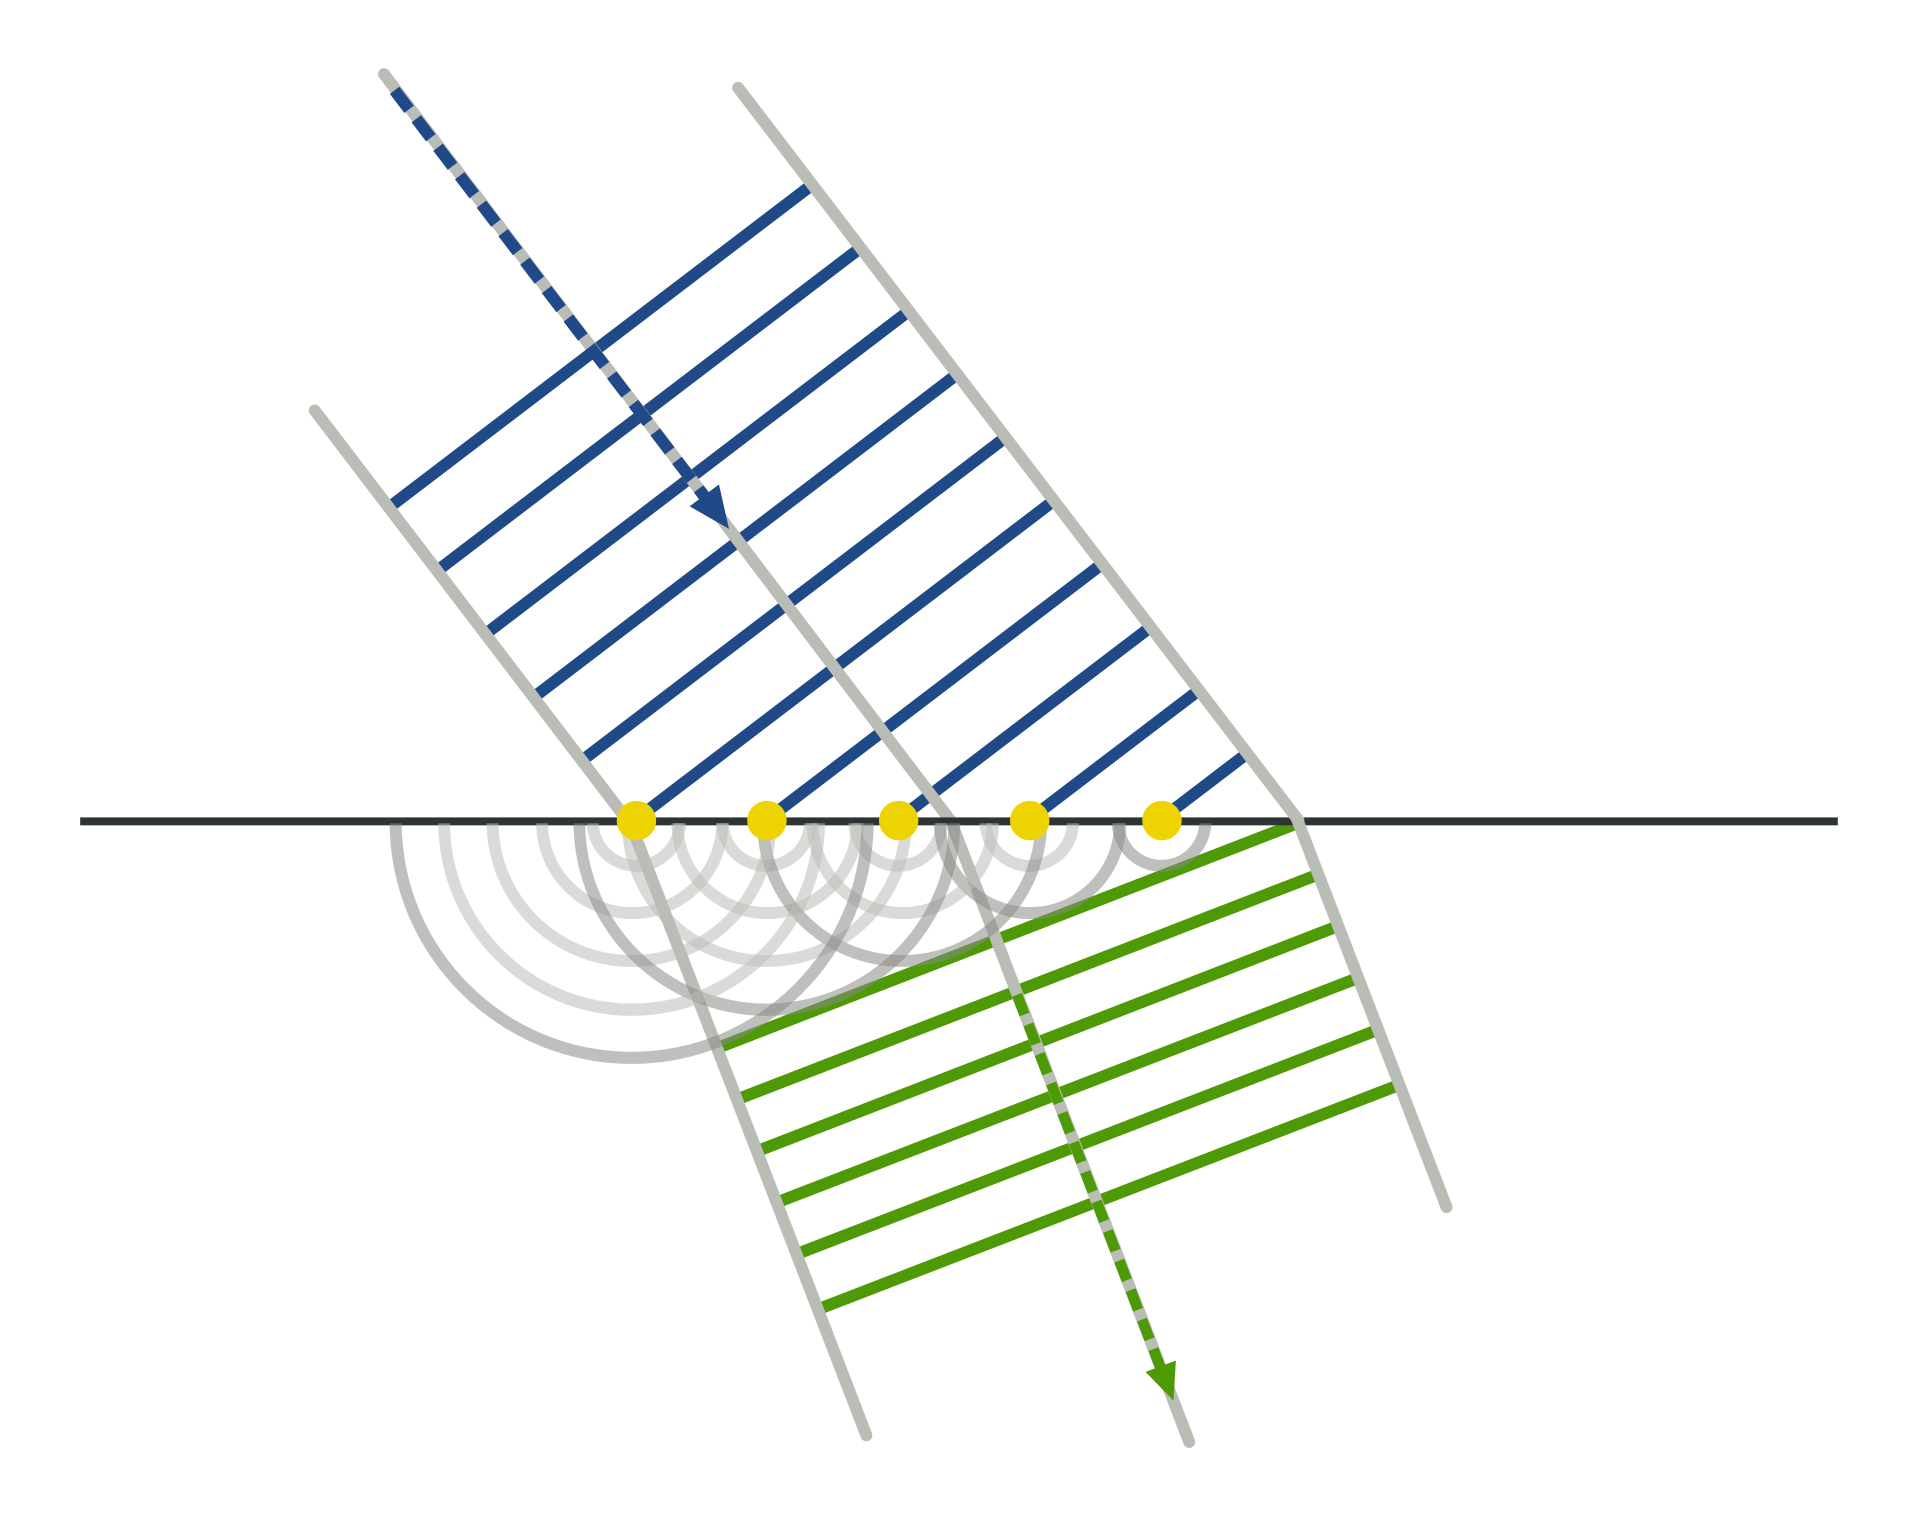
\includegraphics[width = 0.2\textwidth]{Figures/Huygen.png}
\end{center}

\pagebreak

\fat{Orte der Maximalen Verstärkung}:
$\Delta \varphi = n 2 \pi \stackrel{!}{=} k \delta \sin(\alpha)$ mit $\delta$ den Abständen
zwischen den Löchern.

\vspace{1\baselineskip}

\fat{Nullstellen der Intensität}:
Nullstellen: $\frac{k \cdot d}{2} \sin(\alpha) \stackrel{!}{=} n \cdot \pi$

Orte NST: $\sin(\alpha_{NST}) = n \frac{\lambda}{d}$
mit $d=$ Gesammtlänge der Wand, $\alpha=$ Einfallswinkel der Wellenfront.

\vspace{1\baselineskip}

\fat{Beugung} ist die Abweichung vom gradlinigen Strahlenverlauf an Grenzflächen oder
Öffnungen. Sie ist dann wichtig, wenn die Grösse der Öffnung etwa von der Grössenordnung
der Wellenlänge ist.
\begin{center}
    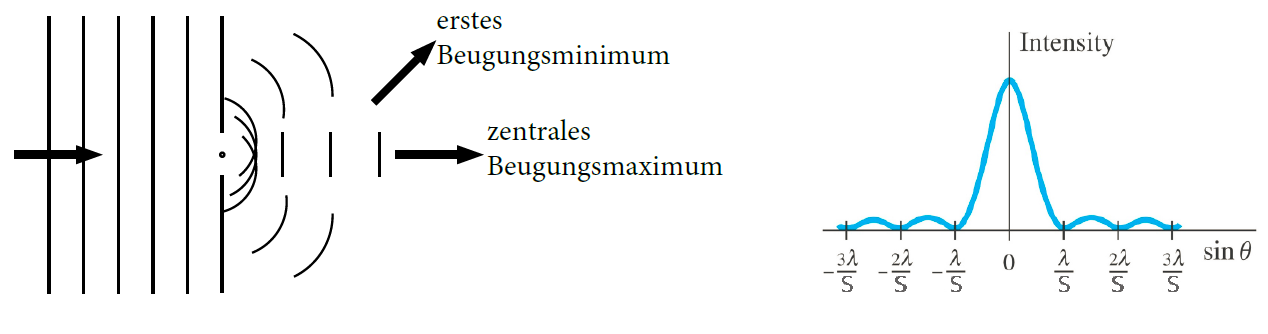
\includegraphics[width=0.4\textwidth]{Figures/Beugung2.png}
    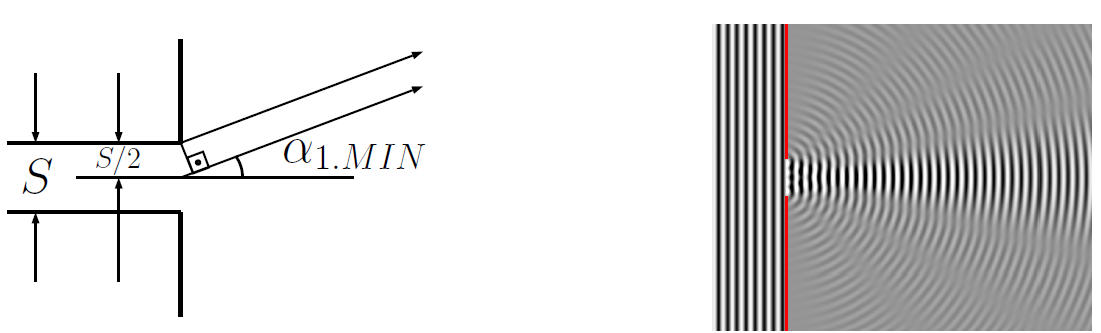
\includegraphics[width=0.3\textwidth]{Figures/Beugung3.png}
\end{center}
Für destruktive Interferenz am ersten Beugungsminimum gilt:
$\frac{S}{2} \sin (\alpha_{1,\min}) = \frac{\lambda}{2} \longrightarrow
\sin (\alpha_{1,\min}) = \frac{\lambda}{S}$

\vspace{1\baselineskip}

\fat{Der Reflexionsgesetz}
Einfallender Lichtstrahl, reflektierter Lichtstrahl und Einfallslot (Oberflächennormale
im Auftreffpunkt) liegen in einer Ebene. Einfallswinkel $\alpha_1$ und Reflexionswinkel
$\alpha_2$ - beide zum Einfallslot hin gemessen - sind gleich.

\vspace{1\baselineskip}

\fat{Das Brechungsgesetz / Snellius'sches Brechungsgesetz}
\begin{align*}
    \frac{\sin(\alpha_1)}{\sin(\alpha_2)} = \frac{c_1}{c_2} =
    \frac{c_{\text{Vakuum}}}{n_1} \frac{n_2}{v_{\text{Vakuum}}}
    = \frac{n_2}{n_1}
    = \frac{v_1}{v_2}
    = \frac{\lambda_1}{\lambda_2}
\end{align*}
mit $n=$ Brechungsindex.

\vspace{1\baselineskip}

\fat{Akustische Linsen}:
Schallgeschw. in einem Gas: $v = \sqrt{\kappa \frac{R T}{M}}$ dabei sind
$\kappa = \frac{C_p}{C_V}$, $R$ die allgemeine Gaskonstante und $M$ die Molekularmasse
des Gases.

\vspace{1\baselineskip}

\fat{Dopplereffekt}
\begin{itemize}
    \item Ruhende Quelle, bewegter Beobachter:
        \begin{itemize}
            \item Beobachter rennt von Quelle weg
                \begin{align*}
                    \nu_B = \nu_Q \klammer{1-\frac{v_B}{\lambda_{\text{emit}} \nu_Q}}
                \end{align*}
            \item Beobachter rennt auf Quelle zu
                \begin{align*}
                    \nu_B = \nu_Q \klammer{1+\frac{v_B}{\lambda_{\text{emit}} \nu_Q}}
                \end{align*}
        \end{itemize}
    \item Ruhender Beobachter, bewegte Quelle:
        \begin{itemize}
            \item Quelle entfernt sich vom Beobachter
                \begin{align*}
                    \nu'_B = \nu'_Q \klammer{1-\frac{v_Q}{\lambda_{\text{emit}} \nu_Q}}^{-1}
                \end{align*}
            \item Quelle bewegt sich auf den Beobachter zu
                \begin{align*}
                    \nu'_B = \nu'_Q  \klammer{1+\frac{v_Q}{\lambda_{\text{emit}} \nu_Q}}^{-1}
                \end{align*}
        \end{itemize}
\end{itemize}

\vspace{1\baselineskip}

\fat{Schockwelle}
Eine Schockwelle breitet sich im \fat{Mach'schen} Kegel aus. Es gilt:
$\vartheta = \arcsin \klammer{\frac{\lambda \nu}{v_Q}}$
Das Verhältnis $\frac{v_Q}{\lambda \nu}$ wird als \fat{Mach'sche Zahl}
bezeichnet.

\vspace{1\baselineskip}

\section{Elektrostatik}

Für den \fat{Strom $I$}, den Zeitintervall $\Delta t$ und der \fat{geflossenen Ladung}
$\Delta Q$ gilt: 
\begin{align*}
    I = \frac{\Delta Q}{\Delta t}
    \quad \text{  ,  } \quad
    \Delta Q = I \cdot \Delta t
\end{align*}

\vspace{1\baselineskip}

\fat{Coulombkraft}:
$Q_1$ wirkt auf $Q_0$:
\begin{align*}
    \vec{F}_{01} = \frac{1}{4 \pi \epsilonnull} \frac{Q_0 Q_1}{(\vec{r}_0 - \vec{r}_1)^2}
                    \frac{\vec{r}_0 - \vec{r}_1}{\abs{\vec{r}_0 - \vec{r}_1}}
\end{align*}

\vspace{1\baselineskip}

\fat{Energie und Ladungsverteilung}
\begin{align*}
    W = \int_{\infty}^{r_{21}} - F_{21} (r) \cdot ds = \frac{1}{4 \pi \epsilonnull} \frac{q_1 q_2}{r_{21}}
\end{align*}

\vspace{1\baselineskip}

\fat{Elektrisches Feld}: $F = q \cdot E$

diskrete Ladungsverteilung:
\begin{align*}
    \vec{E} (\vec{r}) = \frac{1}{4 \pi \epsilonnull} \sum_{i=1}^n \frac{q_i}{(\vec{r} -\vec{r}_i)^2} \frac{\vec{r} - \vec{r}_i}{\abs{\vec{r} - \vec{r}_i}}
\end{align*}
kontinuierliche Ladungsverteilung: ($dq = \rho dV$)
\begin{align*}
    \vec{E} (\vec{r}) = \frac{1}{4 \pi \epsilonnull} \int_V \frac{\rho (\vec{r'})}{(\vec{r}-\vec{r'})^2} \frac{\vec{r} - \vec{r'}}{\abs{\vec{r}-\vec{r'}}} dV'
\end{align*}

\vspace{1\baselineskip}

\fat{Elektrisches Potential}

diskret:
\begin{align*}
    \phi (\vec{r}) = \frac{1}{4 \pi \epsilonnull} \sum_{i=1}^n \frac{q_i}{\abs{\vec{r}-\vec{r}_i}}
\end{align*}
kontinuierliche:
\begin{align*}
    \phi (\vec{r}) = \frac{1}{4 \pi \epsilonnull} \int \frac{1}{\abs{\vec{r}-\vec{r'}}} dq
    = \frac{1}{4 \pi \epsilonnull} \int_V \frac{\rho (\vec{r'})}{\abs{\vec{r}-\vec{r'}}} dV'
\end{align*}

\vspace{1\baselineskip}

\fat{Potential eines Plattenkondensators}: $\phi_{BA} = E \Delta z$

\vspace{1\baselineskip}

\fat{Gauss'sches Gesetz}
\begin{align*}
    d \Phi = E \cdot da \ \ \Longrightarrow \ \ \Phi = \int_{\partial V} E \cdot da
\end{align*}
\begin{align*}
    E = - \nabla \phi
    \quad \text{  ,  } \quad
    \div E = \nabla \cdot E = \frac{\rho}{\epsilonnull}
\end{align*}

\vspace{1\baselineskip}

\fat{Satz von Stokes}
\begin{align*}
    \rot E = 0
\end{align*}

\vspace{1\baselineskip}

\fat{Poisson-Gleichung}
\begin{align*}
    \Delta \phi = - \frac{\rho}{\epsilonnull}
\end{align*}

\vspace{1\baselineskip}

\fat{Laplace-Gleichung}
(Spezialfall $\rho = 0$)
\begin{align*}
    \Delta \phi = 0
\end{align*}

\pagebreak

\fat{Berechnungsmethoden: E-Felder}

\begin{tcolorbox}
    
    \footnotesize{
    \textbf{Rezept: Über das Potential}
    \begin{enumerate}
        \item Ladungselement $dq$ aufschreiben (zB: $dq = \lambda dx$ für eine Linienladung)
        \item Position des Betrachtungspunkts ($\vec{r}$) und des Ladungselements ($\vec{r}'$) aufschreiben
        \item $|\vec{r}- \vec{r}'|$ bestimmen
        \item Alle oben bestimmten Grössen in die Gleichung für das Potential einsetzen
        
        \begin{equation*}
        \Phi = \frac{1}{4 \pi \varepsilon_0}\int \frac{1}{|\vec{r}- \vec{r}'|} dq
        \end{equation*}
        
        \item Integration mit geeigneten Grenzen (zB: Stabanfang bis Stabende)
        \item Benutze  \begin{equation*}
        \Vec{E} = - \nabla \Phi
    \end{equation*} um das elektrische Feld zu finden.
    \end{enumerate}}
    \end{tcolorbox}
\begin{tcolorbox}
    \footnotesize{
    \textbf{Rezept: Direkt über das elektrische Feld}
    \begin{enumerate}
    \item Zeichne deine Anordnung in eine Skizze. Wähle dazu ein geeeignetes Koordinatensystem (2-dim, 3-dim). Betrachte die \textbf{Symmetrien} deiner Skizze. 
    \item Bestimme nun den Ortsvektor $\Vec{r}$ deines Betrachtungspunkts.
    \item Wähle nun ein infinitesimales Ladungselement $dq$ auf deinem Ladungsträger. Beachte dabei, dass es sehr sinnvoll ist, wenn dessen Positionsvektor $\Vec{r}'$ senkrecht auf $\Vec{r}$ steht.
    \item Benutze nun
    
    \begin{equation*}
        d\Vec{E} = \frac{dq}{4 \pi \varepsilon_0} \frac{1}{|\Vec{r}- \Vec{r}'|^2} \frac{\Vec{r}- \Vec{r}'}{|\Vec{r}- \Vec{r}'|}
    \end{equation*}
    
    \noindent und setze alle deine bestimmten Argumente ($dq$, $\Vec{r}$ und $\Vec{r}'$) ein. 
    \item Berechne nun das Integral mit geeigneten Grenzen
    
    \begin{equation*}
        \vec{E} = \int \frac{dq}{4 \pi \varepsilon_0} \frac{1}{|\Vec{r}- \Vec{r}'|^2} \frac{\Vec{r}- \Vec{r}'}{|\Vec{r}- \Vec{r}'|}
    \end{equation*}
    \end{enumerate}}
    \end{tcolorbox}
    
\begin{tcolorbox}
    \footnotesize{
    \textbf{Rezept: Gauss'sches Gesetz}
    
    Als Alternative zum direkten Weg kann man oftmals Symmetrien ausnutzen. Es gilt für den Fluss (Integration über die Oberfläche): 

    \begin{equation*}
        \Phi_E = \int_A \Vec{E} d\Vec{A}
    \end{equation*}
    
    \noindent Gauss'sche Gesetz:
    \begin{equation*}
        \int_A \Vec{E}d\Vec{A} = \frac{Q_{\mathrm{innen}}}{\varepsilon_0} = \frac{1}{\varepsilon_0} \int\rho dV
    \end{equation*}
    
    Wir benutzen dieses Verfahren, wenn folgende Fälle auftreten: Zylindrische oder sphärische Symmetrie, $\infty$-Ebenen}
\end{tcolorbox}{}

\begin{center}
    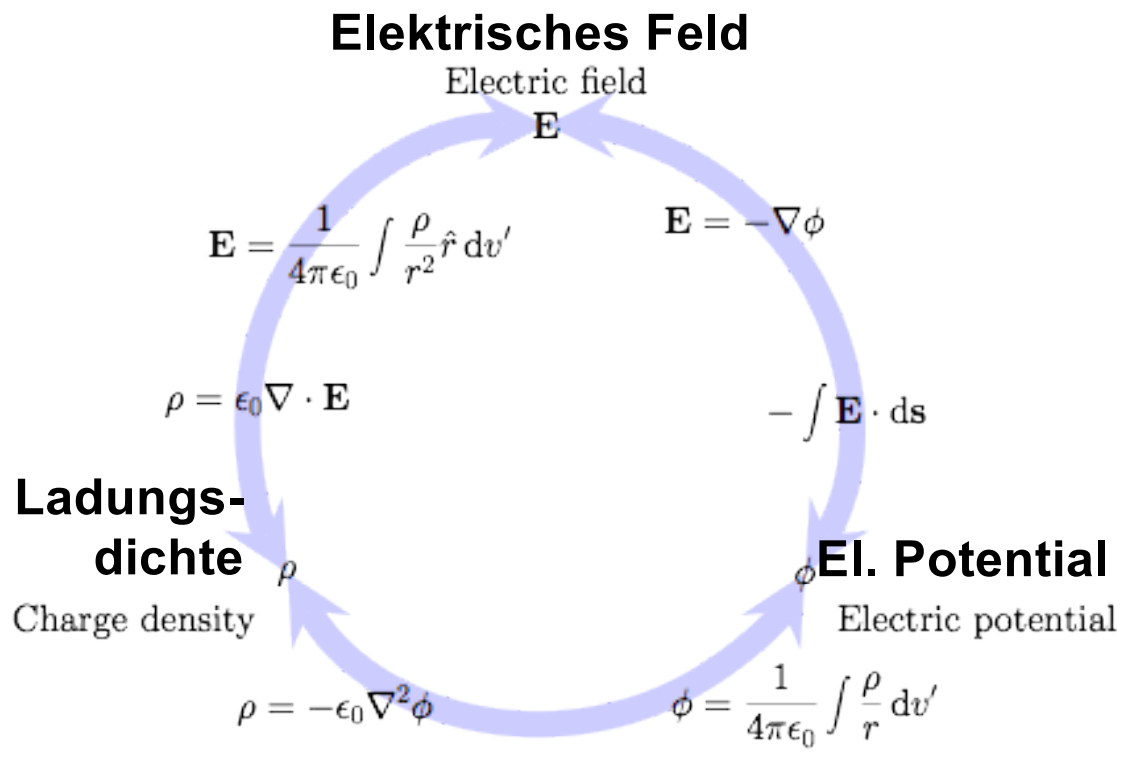
\includegraphics[width=0.4\textwidth]{Figures/Leiter_Isolatoren.png}
\end{center}


\vspace{1\baselineskip}

\section{Elektrische Leiter}

\vspace{1\baselineskip}

\fat{Leiter}:
Einzelnen Ladungen sind sehr mobil. Daher ist das elektrische Feld überall im Leiter Null.
Die Ladungen passen sich also an. Des Weiteren verschwindet die Ladungsdichte überall im
Inneren der Leiters.

\vspace{1\baselineskip}

\fat{Isolator}: Es existieren keine freien Ladungen. Daher können wir das elektrische
Feld und Potential berechnen.

\vspace{1\baselineskip}

\fat{Bedingungen an einen Leiter}:
\begin{itemize}
    \item Das elektrostatische Potential ist überall im Inneren des Leiters auf dessen
            Oberfläche konstant. Insbesondere ist die Oberfläche eine Äquipotentialfläche.
    \item Das elektrische Feld in der Nähe der Oberfläche verschwindet im Inneren und die
            Feldlinien stehen orthogonal auf die Oberfläche.
            $E = \frac{\sigma}{\epsilonnull} \vec{n}$ mit $\sigma =$ lokale Flächenladungsdichte
            auf der Oberfläche und $\vec{n} = $ Normalenvektor.
    \item Die Flächenladungsdichte $\sigma$ ist abhängig von der Form des Leiters.
    \item Die Gesammtladung eines Leiters ist gegeben durch die Integration der Flächenladungsdichte
            über die Oberfläche
            \begin{align*}
                Q = \int_S \sigma da = \epsilonnull \int_S E da
            \end{align*}
\end{itemize}

\vspace{1\baselineskip}

\fat{Das allgemeine elektrostatische Problem}

Wir betrachten einen Leiter im Vakuum, sodass die \fat{Laplacegleichung} zu
$\delta \phi = 0$ wird. Es gibt verschiedene Randbedingungen, die man betrachten kann:
\begin{enumerate}
    \item \fat{Dirichlet-Randbedingung}: Das Potential $\phi$ ist für alle Leiter definiert.
    \item \fat{Neumann-Randbedingung}: Die Ladung $Q$ ist für alle Leiter definiert.
    \item Eine Mischung der beiden.
\end{enumerate}

\vspace{1\baselineskip}

\fat{Eindeutigkeitssatz}:
Falls für eine gegebene Menge an Randbedingungen eine Lösung des elektrostatischen
Problems existiert, so ist diese eindeutig.

\vspace{1\baselineskip}

\fat{Influenz}
Verschiebung von Ladungen in einem Leiter durch eine externe Ladungsverteilung.

\vspace{1\baselineskip}

\fat{Faraday'sche Käfig}
\begin{itemize}
    \item \fat{Ein leerer von einen Leiter umgebener Raum}: Wir wissen, dass das Potential
            auf der Leiteroberfläche konstant sein muss. Damit ist es konstant auf dem ganzen
            Hohlraum, weil er ja keine Ladung einschliesst. Das dabei entstehende elektrische
            Feld ist Null.
    \item \fat{Eine von einem Leiter umgebene Ladung}: Man stelle sich vor, eine positive
            Punktladung $Q$ sitze im Hohlraum eines Leiters. Wegen des Gauss'schen Gesetzes
            muss die Ladung der inneren Oberfläche des Leiters gerade $-Q$ sein
            (Damit das elektrische Feld im Inneren des Leiters wieder Null wird.)
            Die äussere Oberfläche des Leiters trägt dann ebenfalls wieder eine Ladung $Q$,
            damit die Gesammtladung des leiters verschwindet.
    \item \fat{Allgemein}: Durch einen Leiter, der einen Hohlraum umschliesst, wird das
            Innere von allen äussseren Einflüssen abgeschirmt und die Umgebung wird von
            jeglicher Information über die Bewegung der Ladungen im Inneren abgeschnitten.
\end{itemize}


\section{Kondensatoren}

\vspace{1\baselineskip}

\fat{Kapazität} $C$: $[C] = 1 \text{F} = 1 \frac{\text{C}}{\text{V}}$

Es gilt: $Q = C \cdot \phi$, wobei $Q$ die Ladung ist, $C$ die Kapazität und $\phi$ das
Potential (oft auch $U$ oder $V$).

\vspace{1\baselineskip}

\fat{Plattenkondensator}:

\vspace{1\baselineskip}

\begin{minipage}{0.2\textwidth}
    \begin{center}
        \fat{Elektrisches Feld}:
        \begin{align*}
            E_{\text{Plattenkondensator}} = \frac{V}{d}
        \end{align*}
    \end{center}    
\end{minipage}
\begin{minipage}{0.2\textwidth}
    \begin{center}
        \fat{Kapazität}:
        \begin{align*}
            C_{\text{Plattenkondensator}} = \frac{A \epsilonnull}{d}
        \end{align*}
    \end{center}    
\end{minipage}

\vspace{1\baselineskip}

\fat{Gespeicherte Energie}:
\begin{align*}
    dW = \phi dQ = \frac{Q}{C} dQ
    \ \Rightarrow \
    W = \frac{Q^2}{2 C} = \frac{C V^2}{2} = \frac{Q V}{2}
\end{align*}

\vspace{1\baselineskip}

\fat{Ersatzkapazitäten}:
\begin{itemize}
    \item parallel: $C = \sum C_i$
    \item seriell: $\frac{1}{C} = \sum \frac{1}{C_i}$
\end{itemize}
\underline{Bemerkung}: Werden Kondensatoren einfach verbunden, ohne dass es eine
Spannungsquelle gibt, so gelten die Formeln für die Parallelschaltung, da einer der
Kondensatoren als Spannungsquelle fungiert, der andere als Kondensator.


\vspace{1\baselineskip}

\section{Elektrische Ströme}

\vspace{1\baselineskip}

Ein \fat{Elektrischer Strom} entsteht, wenn sich eine Nettoladung in Bewegung befindet.

\vspace{1\baselineskip}

\fat{Stromstärke}:
\[
    I = \frac{dQ}{dt} = \dot{Q} = n A v q
\]
$I$ bezeichnet die Ladung, welche pro Zeit durch einen Leiter fliesst.

\vspace{1\baselineskip}

\fat{Anzahl Ladungsträger}:
\begin{align*}
    \Delta N = n A \Delta x = n A v \Delta t
\end{align*}
$n$ bezeichnet Anzahldichte in $\frac{1}{m^3}$, $A$ Oberfläche des Leiters, $\Delta x$
dessen Länge. Weiter ist $v$ die Driftgeschwindigkeit.

\vspace{1\baselineskip}

\fat{Stromrichtung}
\begin{itemize}
    \item Die \textit{physikalische} Stromrichtung ist die Bewegungsrichtung der Elektronen.
    \item Die \textit{technische / konventionelle} Stromrichtung ist diejenige der positiven Ladungsträger.
\end{itemize}

\pagebreak

\fat{Stromdichte}: $\vec{J} = n q \vec{v}$ \
Allgemeiner:
\begin{align*}
    \vec{J} = \sum_i n_i q_i \vec{v}_i
    \quad \quad \text{  und  } \quad \quad
    I_A = \int \vec{J} \cdot d \vec{A}
\end{align*}
Die Stromdichte gibt uns an, wie viel Strom pro Oberfläche durch den Leiter fliesst.

\vspace{1\baselineskip}

\fat{Ladugserhaltung}:
\begin{align*}
    I = \int_{\partial V} \vec{J} \cdot d \vec{A} = - \int_V \frac{d \rho}{d t} dV
\end{align*}
\fat{Kondinuitätsgleichung}:
\begin{align*}
    \vec{\nabla} \cdot \vec{J} = - \frac{d \rho}{d t}
\end{align*}

\vspace{1\baselineskip}

\fat{Ohm'sches Gesetz}:
\begin{itemize}
    \item \fat{mikroskopisch}: $\vec{J} = \sigma \vec{E}$ mit $\sigma$ der Leitfähigkeit des Materials.
    \item \fat{idealisiert}: $U = R \cdot I$ mit $U$ der Spannung, $R$ dem Widerstand und $I$ dem Strom.
\end{itemize}


\vspace{1\baselineskip}

\section{Schaltkreise}

\vspace{1\baselineskip}

\fat{Kirchhoff'sche Regeln}

\begin{tcolorbox}
    \begin{enumerate}
        \item Für jedes aus Widerständen bestehende Schaltelement gilt das \textbf{Ohm'sche Gesetz}: \begin{equation*}
            V_i = R_i I_i
        \end{equation*}
        
        \item Es dürfen sich keine Ladungen aufbauen, daher gilt \begin{equation*}
            \sum_i I_i = 0
            \quad \quad \text{   resp.  } \quad \quad
            \sum I_{\text{in}} =  \sum I_{\text{out}}
        \end{equation*}
        
        \item Für jede Schleife verschwindet die Summe der Potentialdifferenzen: \begin{equation*}
            \sum_i V_i = 0
        \end{equation*}
    \end{enumerate}
\end{tcolorbox}

\vspace{1\baselineskip}

\fat{Ersatzwiderstände}:
\begin{itemize}
    \item Serieschaltung: $R_{\text{Tot}} = \sum_i R_i$
    \item Parallelschaltung: $\frac{1}{R_{\text{Tot}}} = \sum_i \frac{1}{R_i}$
\end{itemize}

\fat{Ersatzkapazitäten}:
\begin{itemize}
    \item Serieschaltung: $\frac{1}{C} = \sum_i \frac{1}{C_i}$
    \item Parallelschaltung: $C = \sum_i C_i$
\end{itemize}

\vspace{1\baselineskip}

\fat{Energieumwandlung}:

Damit eine Ladung durch einen Schaltkreis fliessen kann, muss eine Energiequelle existieren,
welche die in den Widerständen verlorene Wärme ersetzt. Diese Energiequelle wird auch als
\fat{elektromotorische Kraft} $\mathcal{E}$ bezeichnet.

\pagebreak

\fat{Leistung}:
\begin{align*}
    P = \dot{W} = I U = I^2 R = \frac{V^2}{R}
\end{align*}

\vspace{1\baselineskip}

\fat{Schaltkreise mit Kondensatoren}

Es gilt: $Q = C \cdot V$, wobei $Q$ die Ladung, $C$ die Kapazität und $V$ die Spannung ist.

\vspace{1\baselineskip}

\fat{Entladestrom eines Kondensators}:
\begin{align*}
    I(t) = - \frac{V_0}{R} e^{-\nicefrac{t}{R C}}
\end{align*}
Man nennt $R C$ die \fat{Relaxationsskala}.
Der \fat{Ladestrom} ist analog definiert:
\begin{align*}
    I(t) = \frac{V_0}{R} e^{-\nicefrac{t}{R C}}
\end{align*}

\vspace{1\baselineskip}

\fat{Das Vorzeichen ABC}

\vspace{1\baselineskip}

\begin{minipage}{0.25\textwidth}
    \begin{center}
        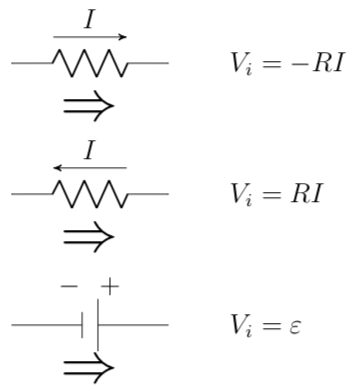
\includegraphics[width=0.8\textwidth]{Figures/Vorzeichen1.png}
    \end{center}
\end{minipage}
\begin{minipage}{0.25\textwidth}
    \begin{center}    
        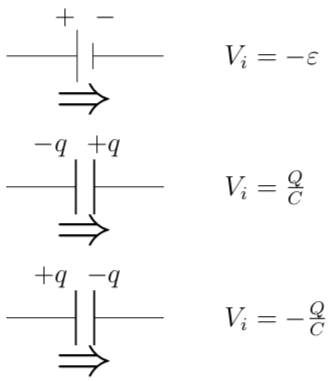
\includegraphics[width=0.8\textwidth]{Figures/Vorzeichen2.png}
    \end{center}
\end{minipage}


\section{Spezielle Relativitätstheorie}

\vspace{1\baselineskip}

\fat{Einstein'sche Postulate}:
\begin{enumerate}
    \item Absolute, gleichförmige Bewegung kann man nicht messen.
    \item Die Geschwindigkeit des Lichts ist unabhängig von Bewegungszustand der Lichtquelle
            Folglich misst jeder Beobachter die gleiche Lichtgeschwindigkeit.
\end{enumerate}

\vspace{1\baselineskip}

\fat{Galilei-Transformation}

Wir verwenden zwei Bezugssysteme $S_A$ und $S_B$ mit den jeweiligen Koordinaten
$x^A , y^A , z^A$ resp. $x^B , y^B , z^B$. $S_B$ bewege sich entlang der positiven
$x$-Achse mit $v_B^A$ relativ zu $S_A$. $S_A$ bewegt sich demnach mit $-v_B^A$ relativ zu
$S_B$. Falls nun die Ursprünge zusammenfallen, so erhalten wir die klassischen Beziehungen:

\begin{minipage}{0.25\textwidth}
    \begin{align*}
        x^A &= x^B + v_B^A t^B \\
        y^A &= y^B \\
        z^A &= z^B \\
        t^A &= t^B
    \end{align*}
\end{minipage}
\begin{minipage}{0.25\textwidth}
    \begin{align*}
        x^B &= x^A - v_B^A t^A \\
        y^B &= y^A \\
        z^B &= z^A \\
        t^B &= t^A
    \end{align*}
\end{minipage}

\vspace{1\baselineskip}

Diese Transformationen verstossen aber gegen die Einstein'schen Postulate.

\pagebreak

\fat{Lorentztransformation}

Die relativistische Transformationsvorschrift (entlang der $x$-Achste) lautet:
\begin{align*}
    x^A &= \gamma (x^B + v_B^{A} t^B) \\
    y^{A} &= y^B \\
    z^{A} &= z^B \\
    t^{A} &= \gamma (t^B + \frac{v_B^{A} x^B}{c^2})
\end{align*}
Dabei ist $\gamma = \frac{1}{\sqrt{1- \beta^2}} > 1$ mit $\beta = \frac{v_B^{A}}{c}  =
\frac{-v_A^B}{c}$

In Matrizenschreibweise heisst das für ein ruhendes System $S$ und ein bewegtes
(in $x$-Richtung) System $S'$:
\begin{align*}
    \begin{pmatrix}
        ct' \\ x' \\ y' \\ z'
    \end{pmatrix} = \begin{pmatrix}
        \gamma (ct - \beta x) \\ \gamma (x- \beta c t) \\ y \\ z
    \end{pmatrix} = \begin{pmatrix}
        \gamma & - \beta \gamma & 0 & 0 \\
        - \beta \gamma & \gamma & 0 & 0 \\
        0 & 0 & 1 & 0 \\
        0 & 0 & 0 & 1
    \end{pmatrix} \begin{pmatrix}
        ct \\ x \\ y \\ z
    \end{pmatrix}
\end{align*}

\vspace{1\baselineskip}

\fat{Zeitdilatation}:
\begin{align*}
    \Delta t^A = \gamma \Delta t^B
    \quad \quad \Longrightarrow \quad \quad
    \Delta t = \gamma \Delta t_{\text{eigen}}
\end{align*}
Das Zeitintervall $\Delta t$ in einem beliebigen Bezugssystem ist stets grösser als die
Eigenzeit.

\vspace{1\baselineskip}

\fat{Längenkontraktion}:
\begin{align*}
    \Delta x^A = \frac{1}{\gamma} \Delta x^B
    \quad \quad \Longrightarrow \quad \quad
    \Delta x = \frac{1}{\gamma} \Delta x_{\text{eigen}}
\end{align*}
Die Länge $l$ in einem beliebigen Bezugssystem ist stets kleiner als die Eigenlänge $l_0$.

\vspace{1\baselineskip}

\fat{Gleichzeitigkeit}

Zwei Ereignisse finden gleichzeitig statt, wenn die von den Ereignissen ausgesandten
Lichtsignale einen Beobachter, der sich in der Mitte der Ereignisse befindet, zus selben
Zeit erreichen.

\vspace{1\baselineskip}

\fat{Invarianz}

Wir definieren das \fat{Raumzeit-Intervall $\Delta s$} als:
\begin{align*}
    \Delta s^2 = c^2 \Delta t^2 - \Delta x^2 - \Delta y^2 - \Delta z^2
\end{align*}
welches eine Invariante der Lorentztransformation ist.
\begin{itemize}
    \item \fat{Zeitartig}: $\Delta s^2 > 0$: Zeitintervalle am kleinsten, wo Ereignisse
            am selben Ort stattfinden
    \item \fat{Raumartig}: $\Delta s^2 < 0$: Länge am kleinsten, wo Raumkoordinate zur
            selben Zeit gemessen
    \item \fat{Lichtkegel}: $\Delta s^2 = 0$: Die Gleichung beschreibt die Ausbreitung
            des Lichtes als Kugelwelle.
\end{itemize}

\vspace{1\baselineskip}

\fat{Geschwindigkeitstransformationen}

Es sei ein Teilchen in $S_B$ mit der Geschwindigkeit $\vec{v} = (v_x , v_y , v_z)^T$.
Die Geschwindigkeit in $S_A$ ist:
\begin{align*}
    v_x^{A} &= \frac{dx^{A}}{dt^{A}} = \frac{\gamma (dx^B + v_B^{A} dt^B)}{\gamma (dt^B + \frac{v_B^{A}}{c^2} dx^B)}
        = \frac{v_x^B + v_B^{A}}{1+\frac{v_B^{A} v_x}{c^2}}
    \\
    v_y^{A} &= \frac{dy^{A}}{dt^{A}} = \frac{v_y^B}{\gamma (1+ \frac{v_B^{A} v_x^B}{c^2})}
    \\
    v_z^{A} &= \frac{dz^{A}}{dt^{A}} = \frac{v_z^B}{\gamma (1+ \frac{v_B^{A} v_x^B}{c^2})}
\end{align*}
wobei $v_B^{A}$ die Geschw. von $B$ im Bezugssystem von $A$ ist.

\vspace{1\baselineskip}

\fat{Relativistischer Dopplereffekt}

Der (longitudale) relativistische Dopplereffekt ist gegeben durch:
\begin{align*}
    \nu^{A} &= \sqrt{\frac{1+\beta}{1-\beta}} \nu^{B}
    \quad \quad \text{für kleiner werdenden Abstand}
    \\
    \nu^{A} &= \sqrt{\frac{1-\beta}{1+\beta}} \nu^{B}
    \quad \quad \text{für grösser werdenden Abstand}
\end{align*}
Der transversale Dopplereffekt ist geg. durch $\nu^{A} = \sqrt{1-\beta^2} \nu^B$

\vspace{1\baselineskip}

\fat{Relativistischer Impuls und relativistische Energie}
\begin{itemize}
    \item \fat{Impuls}: $\vec{p} = \gamma m \vec{v}$
    \item \fat{Energie}: $\Etot = \Ekin + E_0 = \gamma m c^2$ mit $E_0 = mc^2$ der Ruheenergie.
\end{itemize}
Die Masse eines Teilchens ist Lorentz-invariant und es gilt:
\begin{align*}
    E^2 - \vec{p}^2 c^2 = m^2 c^4
\end{align*}

\vspace{1\baselineskip}

\fat{Relativistische Kraft}
\begin{align*}
    m \gamma \vec{v} &= \vec{F} - \frac{1}{c^2} (\vec{F} \cdot \vec{v}) \cdot \vec{v}
    \\
    m \gamma^3 \vec{a} &= (\vec{F} \cdot \hat{v}) \cdot \hat{v}
\end{align*}

\vspace{1\baselineskip}

\fat{Vierer-Impuls}

Energie-Impuls Vektor in $4$er-Koordinaten
\begin{align*}
    P^{\nu} = \begin{pmatrix}
        \nicefrac{\Etot}{c} \\ p_1 \\ p_2 \\ p_3
    \end{pmatrix} = \begin{pmatrix}
        \Etot \\ \vec{p}
    \end{pmatrix}
\end{align*}
\begin{tcolorbox}
    Für einen Vierer-Vektor gilt allgemein:    
    \begin{align*}
        x^\mu = \begin{pmatrix}
        x^0 \\ x^1 \\ x^2\\ x^3
        \end{pmatrix} = \begin{pmatrix}
        x^0 \\ \Vec{x}
        \end{pmatrix}
        \quad \quad \quad
        x_\mu = \begin{pmatrix}
        x_0 \\ x_1 \\ x_2\\ x_3
        \end{pmatrix} = \begin{pmatrix}
        x^0 \\ -x^1 \\ -x^2\\ -x^3
        \end{pmatrix} = \begin{pmatrix}
        x^0 \\ -\Vec{x}
        \end{pmatrix}
    \end{align*}    
    Für das 4er-Skalarprodukt gilt    
    \begin{equation*}
        x^\mu y_\mu = \begin{pmatrix}
        x^0 \\ x^1 \\ x^2\\ x^3
        \end{pmatrix} \cdot \begin{pmatrix}
        y^0 \\ -y^1 \\ -y^2\\ -y^3
        \end{pmatrix} = x^0y^0 - \Vec{x}\cdot \Vec{y}
    \end{equation*}
    Wir nennen $x^{\mu}$ kontravariant und $x_{\mu}$ kovariant.
\end{tcolorbox}


\section{Felder bewegter Ladungen}

\vspace{1\baselineskip}

\fat{Transformationen von elektrischen Feldern an einem Plattenkondensator}
\begin{itemize}
    \item \fat{Elektrisches Feld, senkrecht}: $E'_{\perp} = \frac{\sigma'}{\epsilonnull} =
            \frac{\gamma \sigma}{\epsilonnull} = \gamma E_{\perp}$
    \item \fat{Elektrisches Feld, parallel}: $E'_{\parallel} = \frac{\sigma}{\epsilonnull}
            = E_{\parallel}$
\end{itemize}

\pagebreak

\fat{Transformation von elektrischen Felder einer bewegten Punktladung}

Angenommen wir haben eine Punktladung, die sich mit $v_x$ entlang der $x$-Achse bewegt.
Das elektrische Feld sei in der $xz$-Ebene, also parallel, bzw senkrecht zur Bewegung.
Im mitbewegten Inertialsystem, in dem sich die Ladung im Ursprung und in Ruhe befindet
sind die Komponenten des elektrischen Feldes:
\begin{align*}
    E_x (x,0,z) = \frac{q}{4 \pi \epsilonnull} \frac{x}{(x^2 + z^2)^{\nicefrac{3}{2}}}
    \\
    E_z (x,0,z) = \frac{q}{4 \pi \epsilonnull} \frac{z}{(x^2 + z^2)^{\nicefrac{3}{2}}}
\end{align*}
Mit $r'^2 = x'^2 + z'^2$ und $z' = r' \sin(\theta')$ erhalten wir:
\begin{align*}
    E' = \sqrt{{E'}_x^2 + {E'}_z^2} = \frac{q}{4 \pi \epsilonnull r'^2} \frac{1-\beta^2}{\klammer{1-\beta^2 \sin^2(\theta')}^{\nicefrac{3}{2}}}
\end{align*}
wobei die Striche die Koordinaten im Laborsystem kennzeichnen, welches sich mit
Relativgeschwindigkeit $-v_x$ bewegt.

\vspace{1\baselineskip}

\fat{Kräfte auf bewegte Ladungen}:
\begin{align*}
    F_{\parallel} = F'_{\parallel} = q E'_{\parallel} = q E_{\parallel}
    \quad \quad \quad \quad
    F_{\perp} = \frac{1}{\gamma} F'{\perp} = \frac{1}{\gamma} q E'_{\perp} = q E_{\perp}
\end{align*}


\vspace{1\baselineskip}

\section{Magnetische Felder}

\vspace{1\baselineskip}

Es gilt: $I = \frac{dq}{dt} = \frac{dl}{dt} \frac{dq}{dx} = v \cdot \lambda$
mit $\lambda$ der \fat{Linienladungsdichte}.

\vspace{1\baselineskip}

\fat{Lorentz-Kraft}: Kraft, welche auf bewegte Teilchen in einem Magnetfeld wirkt:
\begin{align*}
    d \vec{F}_L = I (d \vec{l} \times \vec{B}(\vec{r}))
    \quad \text{oder allgemeiner} \quad
    \vec{F} = q \klammer{\vec{E} + \vec{v} \times \vec{B}}
\end{align*}
Mit $I$ Strom, $\vec{B}$ Magnetfeld, $q$ (positive) Ladung des Teilchens,
$E$ elektrisches Feld, $d \vec{r}$ Leiterelement.
\begin{center}
    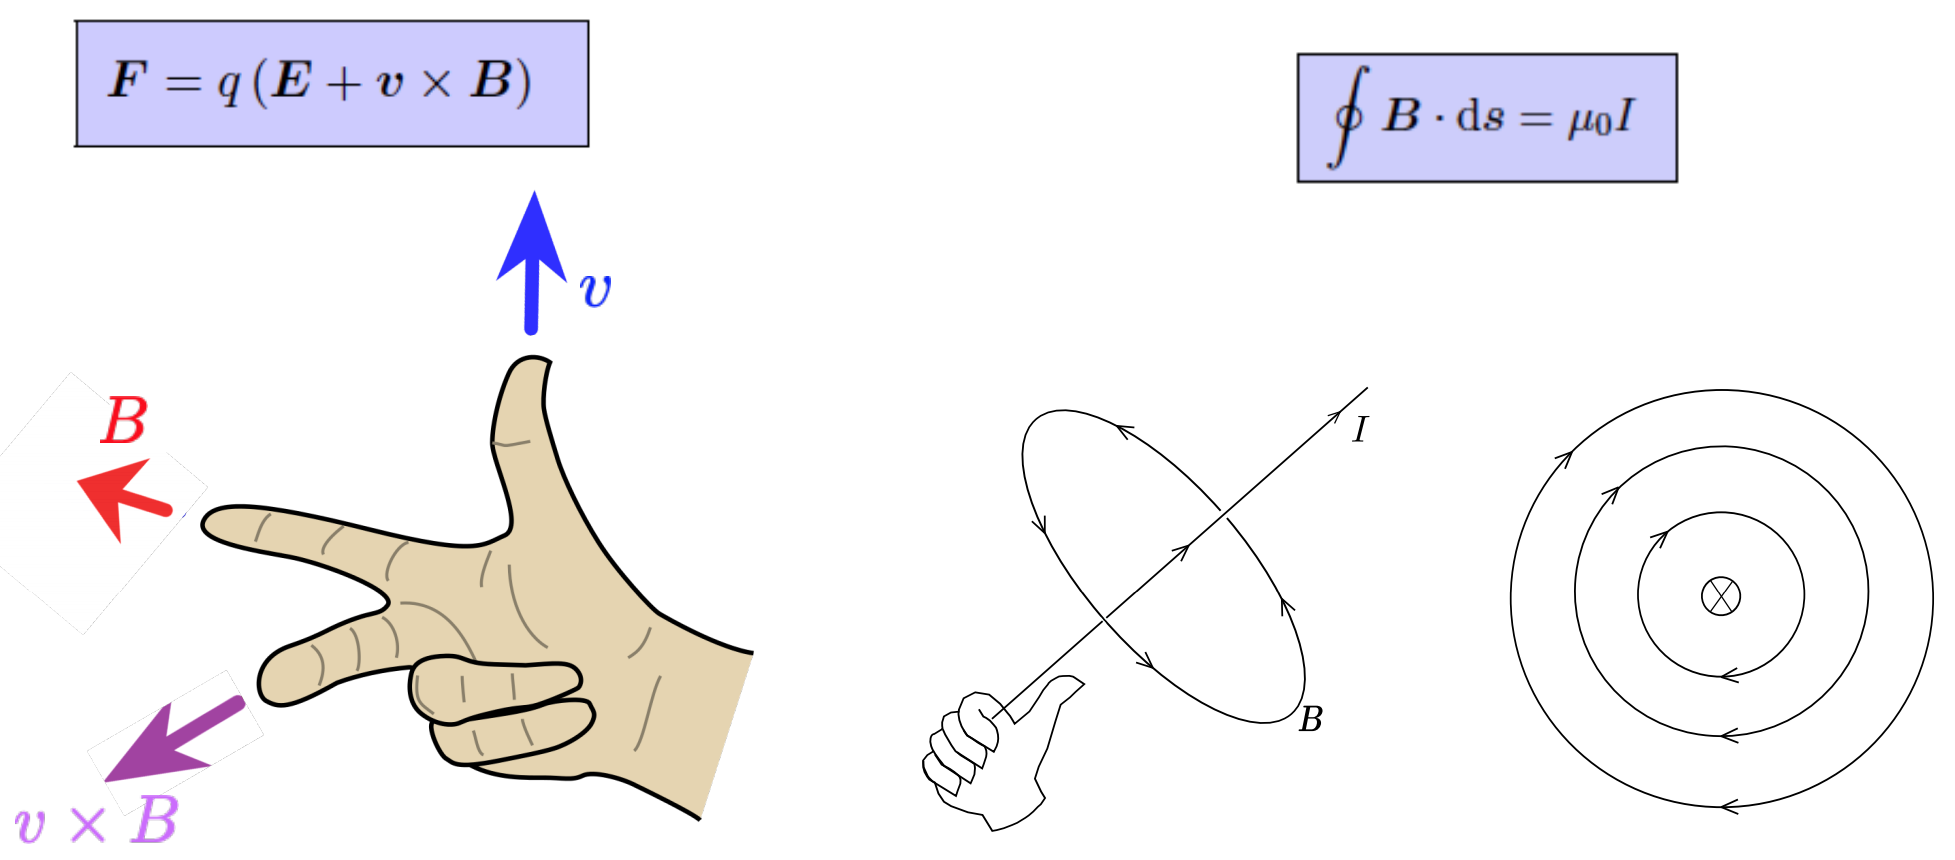
\includegraphics[width=0.4\textwidth]{Figures/3FingerRegel.png}
\end{center}

\vspace{1\baselineskip}

\begin{tcolorbox}
    Das \fat{Ampère'sche Gesetz} wird benutzt, wenn wir unendlich ausgedehnte Leiter haben,
    wie zB einen unendlich langen Draht. Die Formel lautet: 

    \begin{equation*}
        \oint_S \vec{B} \cdot d \vec{s} = \mu_0 I_{\mathrm{eing.}}
        \quad \quad \text{  oder  } \quad \quad
        \vec{\nabla} \times \vec{B} = \munull 
    \end{equation*}

    \subsubsection*{Vorgehen}

    \begin{enumerate}
        \item Skizze zeichnen + Koordinaten wählen
        \item Schleife einzeichnen
        \item Erste Formel für Ampère'sches Gesetz benutzen
        \item Auflösen
    \end{enumerate}
\end{tcolorbox}

\vspace{1\baselineskip}

\fat{Eindeutigkeitssatz}: Für eine gegebene Konfiguration von Strömen $\vec{J}(\vec{r})$
existiert ein eindeutiges Magnetfeld $\vec{B}(\vec{r})$.

\vspace{1\baselineskip}

\fat{Das Vektorpotential} ist definiert als:
\begin{align*}
    \vec{A}(\vec{r}) = \frac{\munull}{4 \pi} \int_{\R^3} \frac{\vec{J}(\vec{r'})}{\abs{\vec{r}-\vec{r'}}} dx' dy' dz'
    \quad \quad \Leftrightarrow \quad \quad \Delta \vec{A} = - \munull \vec{J}
\end{align*}

\vspace{1\baselineskip}

\fat{Das Biot-Savart'sche Gesetz}

\begin{tcolorbox}
    Die Formel von Biot-Savart lautet wie folgt: 
    \begin{equation*}
        d\Vec{B}(\Vec{r}) = \frac{\mu_0}{4 \pi}I d\Vec{l} \times \frac{\Vec{r}- \Vec{r}'}{|\Vec{r}- \Vec{r}'|^3}
        = \frac{\mu_0 I}{4 \pi r^2} (d \vec{l} \times \hat{r})
        = \frac{\mu_0}{4 \pi r^2} (\vec{J} \times \hat{r}) dV
    \end{equation*}
    \begin{align*}
        \vec{B} = \frac{\munull q}{4 \pi r^2} (\vec{v} \times \hat{r})
    \end{align*}
    \begin{itemize}
        \item \textbf{Leiterelement $d\vec{l}$:} \\
        Wir wählen uns auf jedem Leiter ein infinitesimales Leiterelement. Dies beschreiben wir
        dann im gewählten Koordinatensystem. Es beschreibt also einen kleinen Ausschnitt auf dem
        Leiter. Später wird dann über dieses Element integriert.
        \item \textbf{Position des Leiterelements $ \vec{r}'$:} \\
        Der gestrichene Ortsvektor beschreibt die Position des Leiterelements.
        \item \textbf{Position des Betrachtungspunkts P $\vec{r}$:}
        Um das magnetische Feld letzten Ende zu berechnen, betrachten wir einen bestimmten Punkt in
        allgemeinen Koordinaten, dh. wir können ihn überall wählen, jedoch ist manchmal ein
        bestimmter Punkt gefragt und dann vereinfacht sich die Formel.
    \end{itemize}

    \paragraph{Vorgehen:}
    \begin{enumerate}
        \item $d\vec{l}$ definieren
        \item Position von P bestimmen ($\vec{r}$)
        \item Position von $d\vec{l}$ bestimmen ($\vec{r}'$)
        \item Erste Formel von Biot-Savart verwenden
    \end{enumerate}
\end{tcolorbox}

\vspace{1\baselineskip}

\fat{Energiedichte}
\begin{itemize}
    \item des Magnetfeldes: $u_B = \frac{B^2}{2 \munull}$
    \item des elektrischen Feldes: $u_E = \frac{\epsilonnull E^2}{2}$
\end{itemize}

\vspace{1\baselineskip}

\fat{Hall-Effekt}

In Magnetfeldern wirkt auf bewegte Ladungen eine zu ihrer Bewegungsrichtung senkrecht wirkende
Kraft. In einem stromdurchflossenen Leiter schiebt diese Kraft die Ladungsträger auf eine Seite
des Leiters, und es kommt zu einer Ladungstrennung. Zwischen der oberen und der unteren Seite
des Ladungsträgers entsteht dann eine Spannungsdifferenz, die sogenannte \fat{Hall-Spannung}
\begin{align*}
    U_H = E_H b = v_d B b
\end{align*}

\vspace{1\baselineskip}

\fat{Magnetischer Dipolmoment}

Das magnetische Moment einer Leiterschleife ist gegeben durch:
\begin{align*}
    \vec{\mu} = n I \vec{A}
\end{align*}
wobei $n$ die Anzahl Windungen der Leiterschleife ist. Auf eine Leiterschleife wirkt nun ein
Drehmoment, welches gegeben ist durch
\begin{align*}
    \vec{M} = \vec{\mu} \times \vec{B}
\end{align*}

\vspace{1\baselineskip}

\fat{Relativistische Transformationen}

Wir betrachten einen unendlich ausgedehnten Plattenkondensator parallel zur $xz$-Ebene,
welche sich im Laborsystem $K$ mit der geschwindigkeit $v_0$ in $x$-Richtung bewegt.
Sei $K'$ ein Inertialsystem das sich mit $v$ relativ zu $K$ in $x$-Richtung bewegt
($\beta = \frac{v}{c}$).
\begin{align*}
    E'_{\parallel} &= E_{\parallel}
    \quad \quad \quad \quad
    \vec{E'}_{\perp} = \gamma \klammer{\vec{E}_{\perp} + c \vec{\beta} \times \vec{B}_{\perp}}
    \\
    B'_{\parallel} &= B_{\parallel}
    \quad \quad \quad \quad
    \vec{B'}_{\perp} = \gamma \klammer{\vec{B}_{\perp} - \frac{1}{c} \vec{\beta} \times \vec{E}_{\perp}}
\end{align*}
Im Spezialfall $\vec{B} = 0$:
\begin{align*}
    E'_{\parallel} &= E_{\parallel}
    \quad \quad \quad \quad
    \vec{E'}_{\perp} = \gamma \vec{E}_{\perp}
    \\
    B'_{\parallel} &= 0
    \quad \quad \quad \quad
    \vec{B'}_{\perp} = - \gamma \frac{\vec{\beta}}{c} \times \vec{E}_{\perp}
\end{align*}
Wegen $\vec{\beta} \times \vec{E}_{\parallel} = 0$ folgt:
\begin{align*}
    \vec{B'} = - \frac{\vec{\beta}}{c} \times \vec{E'}
\end{align*}


\vspace{1\baselineskip}

\section{Magnetische Induktion}

\vspace{1\baselineskip}

\fat{Der magnetische Fluss} durch eine Oberfläche $\vec{A}$ ist definiert durch
\begin{align*}
    \Phi_{\text{mag}} = \int_A \vec{B} \cdot d \vec{A}
\end{align*}

\vspace{1\baselineskip}

\begin{center} 
    \begin{minipage}{0.15\textwidth}
        \begin{center}
            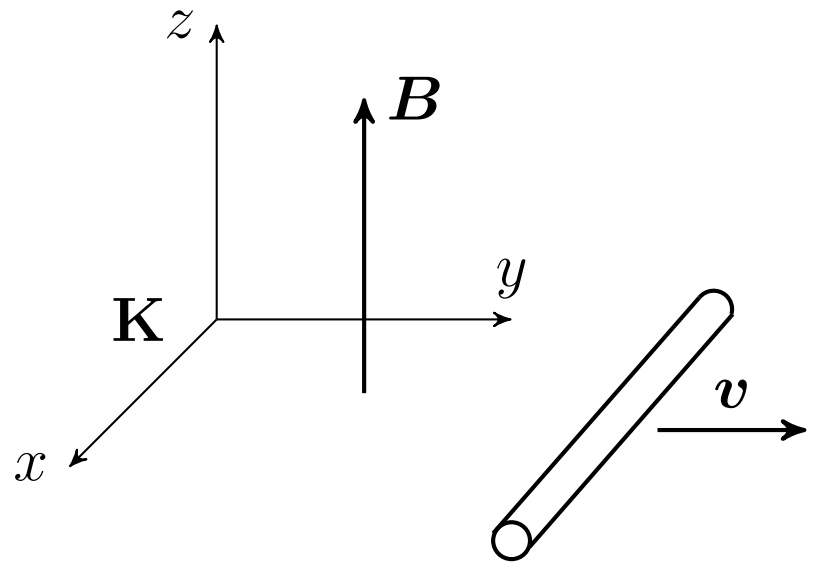
\includegraphics[width=\textwidth]{Figures/Induktion.png}
        \end{center}
    \end{minipage}\hspace{15pt}
    \begin{minipage}{0.3\textwidth}
        In der linken Darstellung gilt für den Stab mit Endpunkten $A$ und $B$:
        \begin{align*}
            U_{BA} = \int_A^B q (\vec{v} \times \vec{B}) \cdot d \vec{s}
        \end{align*}
    \end{minipage}
\end{center}

\vspace{1\baselineskip}

Die \fat{elektromotorische Kraft} ist dann gegeben als:
\begin{align*}
    \mathcal{E} = \oint_C \ (\vec{v} \times \vec{B}) \cdot d \vec{s} = \frac{U_{BA}}{q}
\end{align*}

\vspace{1\baselineskip}

\fat{Faraday'sches Gesetz}:
\begin{align*}
    \mathcal{E} = U_{\text{ind}} = - \frac{d \Phi_{\text{mag}}}{dt}
    = - \frac{d}{dt} \int_A \vec{B} \cdot d \vec{A}
\end{align*}

\vspace{1\baselineskip}

\fat{Das Lenz'sche Gesetz}

Die magnetisch induzierte elektromotorische Kraft erzeugt ihrerseits ein Magnetfeld, das der
Änderung des Flusses entgegenwirkt.

\vspace{1\baselineskip}

\begin{minipage}{0.2\textwidth}
    Die \fat{Leistung}, die eine externe Kraft $\vec{F}_{\text{ext}}$ aufbringen muss, um im
    Widerstand $R$ dissipierte Joul'sche Wärme zu ersetzen, ist gegeben durch
\end{minipage} \hspace{15pt}
\begin{minipage}{0.25\textwidth}
    \begin{center}
        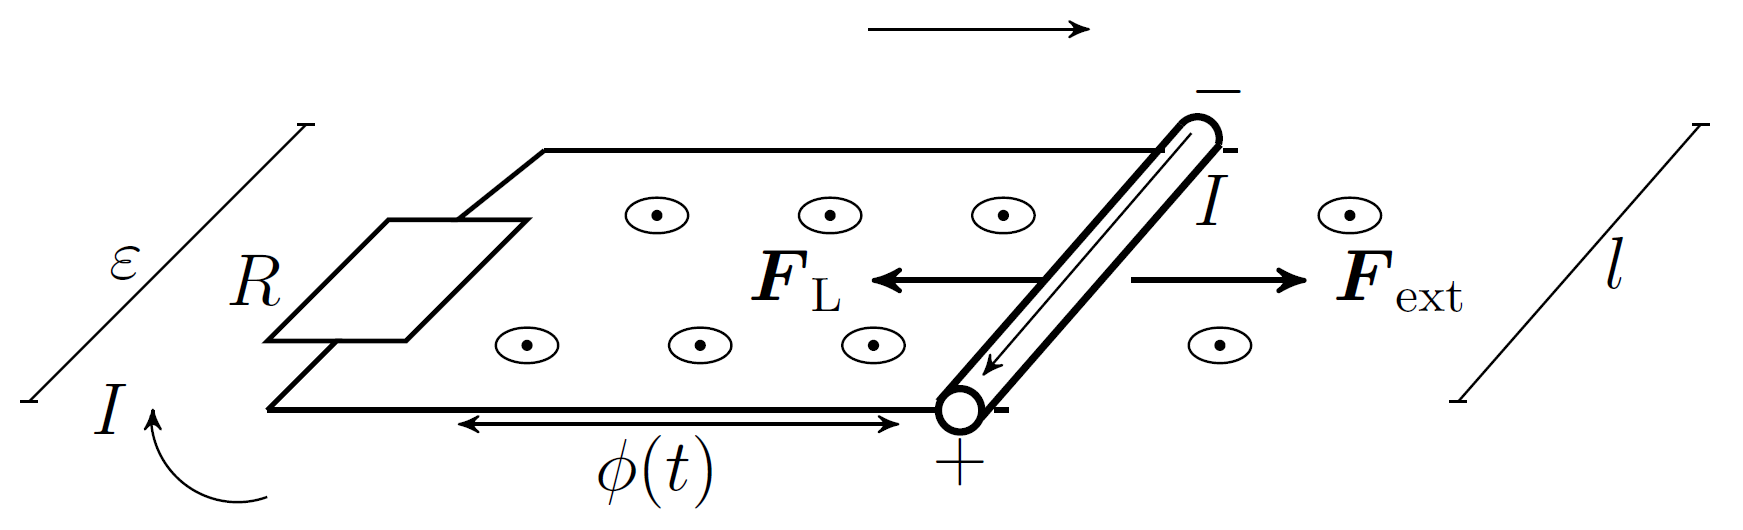
\includegraphics[width=\textwidth]{Figures/Lenz.png}
    \end{center}
\end{minipage}
\begin{align*}
    \vec{F}_{\text{ext}} \cdot \vec{v} = l I B v = \mathcal{E} I
    \quad \quad \quad \quad \quad \quad \text{ für diesen Aufbau}
\end{align*}

\vspace{1\baselineskip}

\fat{Selbstinduktion}

Der Strom durch eine Spule erzeugt ein Magnetfeld. Das Magnetfeld ist proportional zum Strom $I$.
Der magnetische Fluss ist:
\begin{align*}
    \Phi_{\text{mag}} = L I
\end{align*}
mit $L$ der \fat{Selbstinduktivität} der Spule. Die Spannung durch Selbstinduktion
ist nach dem Faraday'schen Gesetz:
\begin{align*}
    U_{\text{ind}} = -L \frac{dI}{dt}
\end{align*}

\vspace{1\baselineskip}

\fat{Gegenseitige Induktivität}
ist der Einfluss auf eine Spule, erzeugt durch eine andere Spule
\begin{align*}
    \Phi_{\text{mag},21} = M_{21} I_1
\end{align*}
mit $M_{21}$ der \fat{gegenseitigen Induktivität}. Es gilt: $M_{12} = M_{21}$

\vspace{1\baselineskip}

Das Magnetfeld einer langen Spule mit einer Querschnittsfläche $A$, Länge $l$ und
Anzahl Windungen $N$ ist gegeben als:
\begin{align*}
    B = \munull \frac{N}{l} I
\end{align*}
Dann folgt:
\begin{align*}
    &\Phi = \munull A \frac{N}{l} I N
    \quad \Longrightarrow \quad
    \mathcal{E}_{\text{ind}} = - \frac{d \Phi}{dt} = - \munull \frac{N^2}{l} A \frac{dI}{dt}
    \\
    &\Longrightarrow L = \munull \frac{A N^2}{l}
\end{align*}

\vspace{1\baselineskip}

\fat{Gespeicherte Energie}:
\begin{align*}
    U = \frac{1}{2} L I^2 = \frac{1}{2 \munull} \int_V B^2 dV
\end{align*}


\vspace{1\baselineskip}

\section{Wechselströme}

\vspace{1\baselineskip}

Da $Q = C V$ folgt: $I = - \frac{dQ}{dt} = -C \frac{dV}{dt}$.

\vspace{1\baselineskip}

\fat{Frei schwindenger gedämpfter $LRC$-Stromkreis}
\begin{itemize}
    \item $\omega_0 = \sqrt{\frac{1}{LC}}$
    \item $\rho = \frac{R}{2L}$
\end{itemize}
\begin{enumerate}
    \item \fat{Schwache Dämpfung}: $\rho^2 < \omega_0^2$ oder $R^2 < 4 \frac{L}{C}$:
            Lösung: $V(t) = V_0 e^{\frac{R}{2L}t} \cos(\omega t)$ \ mit \
            $\omega = \sqrt{\omega_0^2 - \rho^2} = \sqrt{\frac{1}{LC} - \frac{R^2}{4L^2}}$
    \item \fat{Starke Dämpfung}: $\rho^2 > \omega_0^2$ oder $R^2 > 4 \frac{L}{C}$: Lösung:
            $V(t) = A e^{-\beta_1 t} + B e^{- \beta_2 t}$ \ mit \
            $\beta_{1,2} = \frac{R}{2L} \pm \sqrt{\frac{R^2}{4L^2} - \frac{1}{LC}}$
    \item \fat{Sehr starke Dämpfung}: $R^2 >> 4 \frac{L}{C}$: Lösung:
            $V(t) = V_0 e^{- \frac{R}{L} t}$
    \item \fat{Kritische Dämpfung}: $\rho = \omega$ oder $R^2 = 4 \frac{L}{C}$: Lösung:
            $V(t) = A e^{- \frac{R}{2L} t} (1+Bt)$
\end{enumerate}

\vspace{1\baselineskip}

\fat{Zusammenfassung Spannungsabfall}:
\begin{itemize}
    \item Widerstand: $V_R = - I R$
    \item Kondensator: $V_C = \frac{Q}{C}$
    \item Spule: $V_L = - L \frac{dI}{dt}$
\end{itemize}
\fat{Achtung: Vorzeichen sind relativ!}
Beim Kondensator: Ist die Stromrichtung gleich dem Potential\underline{abfall} (von Minus zu
Plus), wo erhalten wir eine parallele Situation. Für die parallele Konfiguration erhalten wir ein
negatives Vorzeichen falls man von \underline{Plus nach Minus} geht! Für den antiparallelen
Fall, haben wir ein positives Vorzeichen.

\vspace{1\baselineskip}

\fat{Verschiedene Stromkreise}:
\begin{itemize}
    \item \fat{$RL$-Stromkreis}: "Strom ist zu Spät, in Induktivität", Lösungen:
            $\tan(\alpha) = - \frac{\omega L}{R}$ und $I_0 =
            \frac{\mathcal{E}_0}{\sqrt{R^2 + \omega^2 L^2}}$
    \item \fat{$RC$-Stromkreis}: "Strom eilt vor, am Kondensator", Lösungen:
            $\tan(\alpha) = \frac{1}{\omega R C}$ und $I_0
            \frac{\mathcal{E}_0}{\sqrt{R^2 + \frac{1}{\omega^2 C^2}}}$
    \item \fat{$RLC$-Schwingkreis}: Lösungen: $\tan(\alpha) = - \frac{\omega L'}{R}$ mit
            $L' = \omega L - \frac{1}{\omega C}$ und $I_0 =
            \frac{\mathcal{E}_0}{\sqrt{R^2 + \klammer{\omega L - \frac{1}{\omega C}}^2}}$

            Maximales $I_0$ bei $\omega_{\text{max}} = \frac{1}{\sqrt{LC}}$.

            Der dimensionslose \fat{Qualitätsfaktor} ist: $\mathcal{Q} = \frac{L \omega_{\text{max}}}{R}
            = \frac{1}{R} \sqrt{\frac{L}{R}}$
\end{itemize}

\vspace{1\baselineskip}

Bei hoher Frequenz des Wechselstromes setzt ein Kondensator dem Stromfluss nahezu keinen
Widerstand entgegen.

\vspace{1\baselineskip}

\fat{Beschreibung durch komplexe Zahlen}:

\begin{itemize}
    \item \fat{elektromotorische Kraft}: $\mathcal{E} (t) = \mathcal{E}_0 e^{i \omega t}$
    \item \fat{komplexe Strom}: $I = I_0 e^{i (\omega t + \alpha)}$
    \item $\alpha = \arctan \klammer{\frac{\Im (I)}{\Re (I)}} =
            \arctan \klammer{\frac{\Im (Y)}{\Re (Y)}}$
    \item \fat{Admittanz}: $Y$: Verallgemeinerung des Leitwertes in Gleichstromkreisen,
            es gilt: $I = Y V$.
    \item \fat{Impedanz}: $Z$: Verallgemeinerung des Ohm'schen Widerstandes, es gilt:
            $Z = \frac{1}{Y} \ \Rightarrow \ V = Z I$.
\end{itemize}

Bei einer \fat{Parallelschaltung} gilt: $Y = \sum_j Y_j$

\vspace{1\baselineskip}

Bei einer \fat{Serienschaltung} gilt: $Z = \sum_j Z_j$

\pagebreak

\begin{center}
    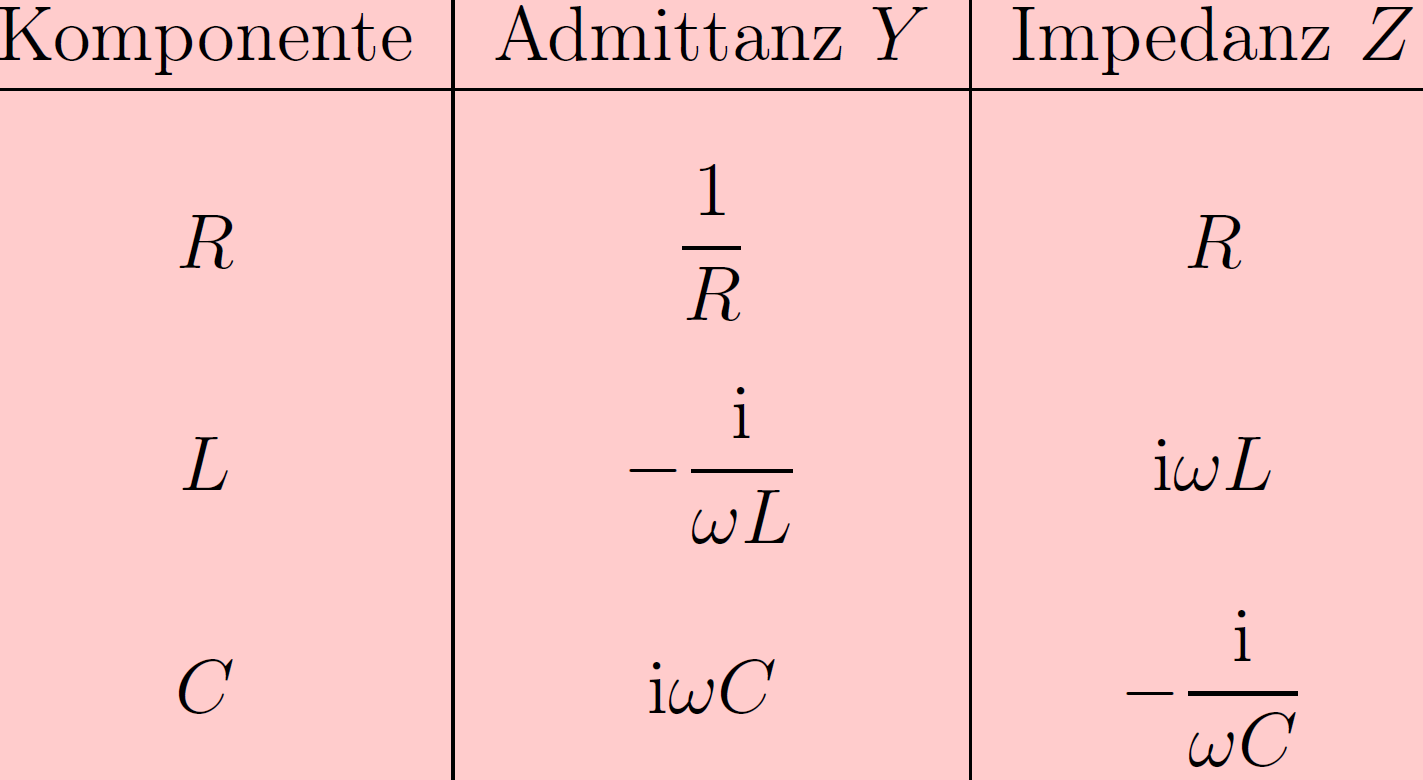
\includegraphics[width=0.3\textwidth]{Figures/Komplex.png}
\end{center}

\vspace{1\baselineskip}

\fat{Leistungsaufnahme eines Stromkreises}

\begin{itemize}
    \item $P = I V$
    \item $\Re (IV) \neq \Re(I) \Re(V)$
    \item Mittlere Leistung: $\langle P \rangle = \langle V I \rangle = \frac{1}{T} \int_0^T V(t) I(t) dt$
    \item \fat{Effektivwerte}: $V_{\text{eff}} = \sqrt{\langle V^2 \rangle}$ und
            $I_{\text{eff}} = \sqrt{\langle I^2 \rangle}$
\end{itemize}


\vspace{1\baselineskip}

\section{Maxwellgleichungen und elektromagnetische Wellen}

\vspace{1\baselineskip}

\fat{Maxwellgleichungen}:
\begin{enumerate}
    \item $\vec{\nabla} \cdot \vec{E} = \frac{\rho}{\epsilonnull}$ \quad (Gauss/Coulomb)
    \item $\vec{\nabla} \cdot \vec{B} = 0$ \quad (Nicht-Existenz von magnetischen Monopolen)
    \item $\vec{\nabla} \times \vec{E} = - \frac{\partial \vec{B}}{\partial t}$ \quad (Faraday'sches Gesetz)
    \item $\vec{\nabla} \times \vec{B} = \munull \vec{J} + \munull \epsilonnull \frac{\partial \vec{E}}{\partial t}$
            \quad (Ampèr'sches Gesetz)
    \item $\vec{\nabla} \cdot \vec{J} = - \frac{\approx \rho}{\partial t}$ \quad (Kontinuitätsgleichung)
\end{enumerate}
In Integralform:
\begin{align*}
    &\int_A \vec{E} d \vec{A} = \frac{q_{\text{innen}}}{\epsilonnull} \\
    &\int_A \vec{B} d \vec{A} = 0 \\
    &\oint_C \vec{E} d \vec{l} = - \frac{d}{dt} \int_A \vec{B} d \vec{A} \\
    &\oint_C \vec{B} d \vec{l} = \munull I + \munull \epsilonnull \int \frac{\partial \vec{E}}{\partial t} d \vec{A}
\end{align*}

\vspace{1\baselineskip}

\fat{Die \underline{homogene} Wellengleichung und deren Lösungen}:
Im Vakuum: $\rho = 0$ und $\vec{J} = 0$ $\Rightarrow$ \fat{homogene Maxwellgleichungen}:
\begin{enumerate}
    \item $\vec{\nabla} \cdot \vec{E} = 0$
    \item $\vec{\nabla} \cdot \vec{B} = 0$
    \item $\vec{\nabla} \times \vec{E} = - \frac{\partial \vec{B}}{\partial t}$
    \item $\vec{\nabla} \times \vec{B} = \munull \epsilonnull \frac{\partial \vec{E}}{\partial t}$
\end{enumerate}

\pagebreak

\fat{Elektromagnetische Wellen}:
\begin{itemize}
    \item Es gilt $\abs{\vec{E}} = c \cdot \abs{\vec{B}}$
    \item Elektromagnetische Wellen breiten sich mit Lichtgeschwindigkeit $c =
            \frac{1}{\sqrt{\epsilonnull \munull}}$ aus und das Licht ist eine elektromagnetische
            Welle.
    \item Das elektrische und magnetische stehen orthogonal zueinander und zur Ausbreitungsrichtung.
            Insbesondere gilt: $\vec{E} = \vec{B} \times c \hat{k}$ oder $\vec{B} =
            \frac{\vec{k}}{\omega} \times \vec{E}$ \ \ wobei $\hat{k}$ der Einheitsvektor in
            der Ausbreitungsrichtung der Welle ist.
\end{itemize}

\vspace{1\baselineskip}

Der \fat{Pointing-Fluss} ist $S = \frac{1}{\munull} \langle E B \rangle$ und allgemeiner ist
der \fat{Pointing-Vektor} (Vektorielle Energieflussdichte):
\begin{align*}
    \vec{S} = \frac{1}{\munull} \vec{E} \times \vec{B}
\end{align*}
Der Betrag $\abs{\vec{S}}$ ist gerade die Intensität.

\vspace{1\baselineskip}

\fat{Pointing-Theorem}:

Wenn $\vec{S}$ der Pointing-vektor ist und $u_{em}$ die Energiedichte, dann gilt:
\begin{align*}
    \frac{\partial(u_{mech} + u_{em})}{\partial t} + \vec{\nabla} \cdot \vec{S} = 0
\end{align*}
Im Vakuum gilt:
\begin{align*}
    \frac{\partial u_{em}}{\partial t} + \vec{\nabla} \cdot \vec{S} = 0
\end{align*}

\vspace{1\baselineskip}

Elektromagnetische Wellen sind invariant unter beliebiger Lorentz-Transformation.

\vspace{1\baselineskip}

\fat{Wellengleichung für Potentiale}:
\begin{align*}
    \vec{B} = \vec{\nabla} \times \vec{A}
    \quad \quad \text{  und  } \quad \quad
    \vec{E} = - \frac{\partial \vec{A}}{\partial t} - \vec{\nabla} \phi
\end{align*}
mit $\phi$ dem elektrischen Potential.

\vspace{1\baselineskip}

\fat{Lorenz-Eichung}:
\begin{align*}
    \vec{\nabla} \cdot \vec{A} = - \epsilonnull \munull \frac{\partial \phi}{\partial t}
    \quad \quad \Longrightarrow \quad \quad
    \Delta \phi - \epsilonnull \munull \frac{\partial^2 \phi}{\partial t^2} = \frac{\rho}{\epsilonnull}
\end{align*}

\vspace{1\baselineskip}

\fat{Wellengleichung für das Vektorpotential}
\begin{align*}
    \Delta \vec{A} - \epsilonnull \munull \frac{\partial^2 \vec{A}}{\partial t^2} = - \munull \vec{J}
\end{align*}

\vspace{1\baselineskip}

\fat{D'Alembert Operator}:
$\Box := \Delta - \epsilonnull \munull \frac{\partial^2}{\partial t^2}$

\vspace{1\baselineskip}

\fat{Retardierte Potentiale}
\begin{align*}
    \vec{A} (\vec{r},t) = \frac{\munull}{4 \pi} \int_{\R^3} \frac{\vec{J} (\vec{r'} , t- \nicefrac{\abs{\vec{r}-\vec{r'}}}{c}}{\abs{\vec{r}-\vec{r'}}} dV'
\end{align*}

\vspace{1\baselineskip}

\fat{Der Hertz'sche Dipol}:
\begin{itemize}
    \item Der \fat{Dipolmoment} ist $\vec{P} = Q \cdot \vec{l}$ oder $p(t)=p_0 \sin(\omega t)$ mit:
    \item Variierende Ladung: $Q(t) = Q_0 \sin(\omega t)$
    \item Strom $I(t) = I_0 \cos(\omega t)$ wobei $I_0 = \omega Q_0 = \frac{\omega p_0}{l}$

    \pagebreak

    \item \fat{Momentaner Energietransport} durch \underline{Kugelschale A}:
            \begin{align*}
                P = \int_A \frac{1}{\munull} (\vec{E} \times \vec{B}) \cdot d \vec{a}
            \end{align*}
\end{itemize}


\section{Elektrische und magnetische Felder im Materie}

\vspace{1\baselineskip}

\fat{Dielektrika}:

In einem Material gilt für die Kapazität eines Plattenkondensators: $C = \epsilon C_{\text{Vak}}$
mit $\epsilon$ der \fat{Dielektrizitätskonstante}. Falls Ladungs $Q_0$ konstant ist, gilt:
$V = \frac{1}{\epsilon} V_{\text{Vak}}$. Falls die Spannung $V_0$ konstant ist, gilt:
$Q = \epsilon Q_{\text{Vak}}$.

\vspace{1\baselineskip}

Materialien, welche unabhängig von externen Feldern magnetisch sind, heissen \fat{ferromagnetisch}.
Während \fat{paramegnetische} Materialien das vorhandene Magnetfeld verstärken, wird es durch
\fat{diamagnetische} Materialien abgeschwächt.

\vspace{1\baselineskip}

\fat{Nettokraft in einem inhomogenen Feld}:
\begin{align*}
    \vec{F} = - \vec{\nabla} U = \vec{\nabla} (\vec{p} \cdot \vec{E})
    = \klammer{\vec{p} \cdot \vec{\nabla}} \cdot \vec{E}
    = \begin{pmatrix}
        p_x \ \partial_x E_x \\ p_y \ \partial_y E_y \\ p_z \ \partial_z E_z
    \end{pmatrix}
    = \vec{p} \cdot \begin{pmatrix}
        \nabla E_x \\ \nabla E_y \\ \nabla E_z
    \end{pmatrix}
\end{align*}
\begin{align*}
    &F_x = \vec{p} \cdot \nabla E_x \\
    \Longrightarrow \hspace{20pt} &F_y = \vec{p} \cdot \nabla E_y \\
    &F_z = \vec{p} \cdot \nabla E_z
\end{align*}

\vspace{1\baselineskip}

\fat{Die elektrische Flussdichte und das Gauss'sche Gesetz im Dielektrikum}:

\begin{align*}
    \vec{\nabla} \cdot \vec{E} &= \frac{\rho_{\text{ges}}}{\epsilonnull} =
    \frac{\rho_{\text{frei}} + \rho_{\text{geb}}}{\epsilonnull} =
    \frac{1}{\epsilon} \vec{\nabla} \cdot \vec{E}_{\text{vak}} =
    \frac{\rho_{\text{frei}}}{\epsilon \epsilonnull} =
    \epsilon \vec{\nabla} \cdot \vec{E} + \frac{\rho_{\text{geb}}}{\epsilonnull}
    \\ &=
    \frac{- \rho_{\text{geb}}}{\epsilonnull \cdot (\epsilon -1)}
    \\ \\
    \Longrightarrow \vec{P} &= \epsilonnull (\epsilon -1) \vec{E}
    \quad \quad \Longrightarrow \quad
    \rho_{\text{geb}} = - \vec{\nabla} \cdot \vec{P}
\end{align*}
Wir definieren die \fat{elektrische Flussdichte} oder \fat{dielektrische Verschiebung $D$} durch:
\begin{align*}
    \vec{D} = \epsilonnull \vec{E} + \vec{P}
\end{align*}
Damit folgt das \fat{modifizierte Gauss'sche Gesetz}
\begin{align*}
    \vec{\nabla} \cdot \vec{D} = \rho_{\text{frei}}
\end{align*}
und $\vec{D} = \epsilon \epsilonnull \vec{E}$.

\vspace{1\baselineskip}

Die elektrischen Dipole ($\vec{p}$) erzeugen eine Polarisation $\vec{P}$ welche das externe
$E$-Feld im Material schwächen: $\mathcal{E} = \frac{E_{\text{vak}}}{E_{\text{result}}} \geq 1$.

\vspace{1\baselineskip}

Mit der Teilchendichte $N$ und dem magnetischen Dipolmoment $\mu$ definieren wir die
\fat{Magnetisierung} als $\vec{M} = N \cdot \vec{\mu}$.

\vspace{1\baselineskip}

Wir definieren das \fat{$H$-Feld} als $\vec{H} = \frac{\vec{B}}{\munull} - \vec{M}$.
Es gilt:
\begin{align*}
    \vec{\nabla} \times \vec{H} &= \frac{\partial \vec{D}}{\partial t} + \vec{J}_{\text{frei}} \quad \quad \text{(Ampèr'sches Gesetz in Materie)}
    \\
    \vec{B} &= \munull \mu \vec{H}
\end{align*}


\end{document}